\documentclass{article}

\usepackage{color}
\usepackage{cite}
\usepackage{float}
\usepackage{graphicx}
\usepackage{pgfgantt}
\usepackage{setspace}

\linespread{1.5}
\begin{document}

\begin{titlepage}
	\begin{center}
		\begin{spacing}{1.5}
			\huge{\textbf{Telemetry-based Optimisation for User Training in Racing Simulators}}
		\end{spacing}
		
		\LARGE{François Buhagiar}
		\vspace{5mm}\\
		
\includegraphics[scale=4]{images/UOM_Logo}
		
		\begin{spacing}{1.5}
			\huge{\textbf{Department of Computer Information Systems\\
			\vspace{5mm}
				University of Malta\\
				March 2016 }}
		\end{spacing}
	
		\Large \vfill Submitted in partial fulfilment of the requirements for the degree of B.Sc. (Hons.)
		\clearpage
	\end{center}
\end{titlepage}

\pagenumbering{roman} 

\newpage
\pagenumbering{arabic} 
\setcounter{page}{1}

\newpage
\begin{abstract}
	
%Computer-assisted learning is known to be an effective tool for improving learning in both adults and children. Recent years have seen the emergence of the so-called ‘serious games (SGs)’ that are flooding the educational games market. In this paper, the term ‘serious games’ is used to refer to video games (VGs) intended to serve a useful purpose. The objective was to review the results of experimental studies designed to examine the effectiveness of VGs and SGs on players' learning and engagement. After pointing out the varied nature of the obtained results and the impossibility of reaching any reliable conclusion concerning the effectiveness of VGs and SGs in learning, we stress the limitations of the existing literature and make a number of suggestions for future studies.

This project will be looking into applying serious games in the training of motorsports race drivers. The goal is to improve a driver's lap times in a simulation race game via a pedagogic feedback system. Researching serious games, techniques employed by racing drivers on track, racing simulation games and hardware, will be the foundations for the user case study which is to be carried to evaluate the effectiveness of the developed system
\end{abstract}

\newpage
\section{Acknowledgements}

Luke for racing rig

Keith and Sandro

\newpage
\tableofcontents

\newpage
\section{Other tables and lists}
\listoffigures

\newpage
\section{Table of abbreviations}

\newpage
\section{Introduction}

• Introduce the area and the FYP without assuming that the reader has any special knowledge in the area.
• The aims and goals of the project.
• Any non-aims of the project (e.g. in a purely theoretical project, the development of an artifact would not necessarily be an aim).
• The approach used.
• Any assumptions.
• A high level description of the project.

The gamification of areas of activity such as marketing, problem solving and education \cite{michael2005serious} has validated the use of serious games beyond their initial military use in training strategic skills \cite{djaouti2011classifying}.  Serious games simulate real-world processes designed for the purpose of solving a problem, making their main purpose that of training or educating users. Their popularity has been steadily increasing, as has their adoption, with military \cite{djaouti2011classifying} and emergency service providers (e.g. firefighters \cite{michael2005serious}) employing them to train for specific scenarios that might be encountered on the respective jobs. Motorsports cover a broad range of activities and vehicles, and as with all major forms of sporting activities, require training and dedication, with a pedagogic aspect arising in rote learning and mentoring by experts. The arenas in which motorsport events take places are called circuits; there is a large selection of the latter, ranging from purposely built race tracks to public roads to natural formations such as hills and quarries. There is also a diverse selection of vehicles that take part in motorsports, with the greatest demarcation existing between motorbikes and cars. The focus of this dissertation is that of unifying serious games and motorsport racing; specifically, it will try to show whether a serious game is a powerful enough pedagogical tool that can be used to tangibly improve the performance of race drivers. The scope of the project is limited to four-wheeled cars racing on purposely-built confined circuits with a smooth tarmac surface.  

\subsection{Motivation}
The training process for race drivers has stabilised during the last decade, with rote learning playing a very important part. Starting at an early age, a driver would compete in lower leagues, such as go karting, and undergo training that is mostly founded on trial and error. A mentor, or coach, would correct obvious mistakes and suggest ways for improvement based on experiential knowledge and related literature. The extensive hours of practice serve to hone the skills of a driver and help in the acquisition of the same experiential knowledge of the mentor. Such learning methodology is very resource consuming in that it requires both time and money; often it is geographically-constrained as well, where no suitable training track is available in the locality of the driver. Although simulators, such as those employed by professional racing teams, have helped mitigating traveling and car setup times, they are inadequate for use in more amateurish environments due to cost and logistical problems: setting up such a simulator requires adequate space seldom available to everyone. Democratising the learning process such that proper car control and racing techniques can be mastered by a larger demographic an important motivation behind this work.

\subsection{Why the problem is non-trivial}
The problem at hand is best described as an optimisation problem. Telemetry data provided by the car instrumentation system can be analysed to help identify driving patterns, specifically car-handling mistakes. The identification of these behaviours, which traditionally employs pattern recognition techniques, represents a challenge in itself. Behaviour recognition is key to providing corrective measures in order to improve the driving performance of a given user. In particular, it is the starting point in building a model which maps telemetry data to corrective measures for presentation to the user in real-time and deferred fashion, where even the visualisation of feedback is critical to the success of such a system.

\newpage
\chapter{Background}
\label{sec:background}

This chapter introduces motorsport racing and a number of related concepts that are essential in gaining an understanding of this work. The chapter opens with a brief overview of the sport, followed by an exposition of important concepts like the \emph{racing line}, cornering and braking. A discussion ensues, wherein \emph{understeer} and \emph{oversteer} are explained. A short overview of telemetry is then provided. The chapter concludes with a general introduction to simulation racing rigs.

\section{Motorsport Racing}
In sports, individuals or groups compete to be the first to achieve a particular objective. In circuit motorsport racing, motorised vehicles go round a course for a set number of times. There are varies racing disciplines or series, each one having its own specific rules. However, at the core, participants in all disciplines aim to complete a full lap of the circuit in the shortest time. Some disciplines focus on achieving one fast lap, such as time trials, while others focus on achieving the least amount of time across a fixed number of laps, such as FIA's Formula 1 series. This dissertation will focus on one such discipline, that of confined car racing, which takes place on smooth asphalt surfaces in purpose-built race tracks. 

\begin{figure}
	\centering
	\begin{minipage}{0.45\textwidth}
		\centering
		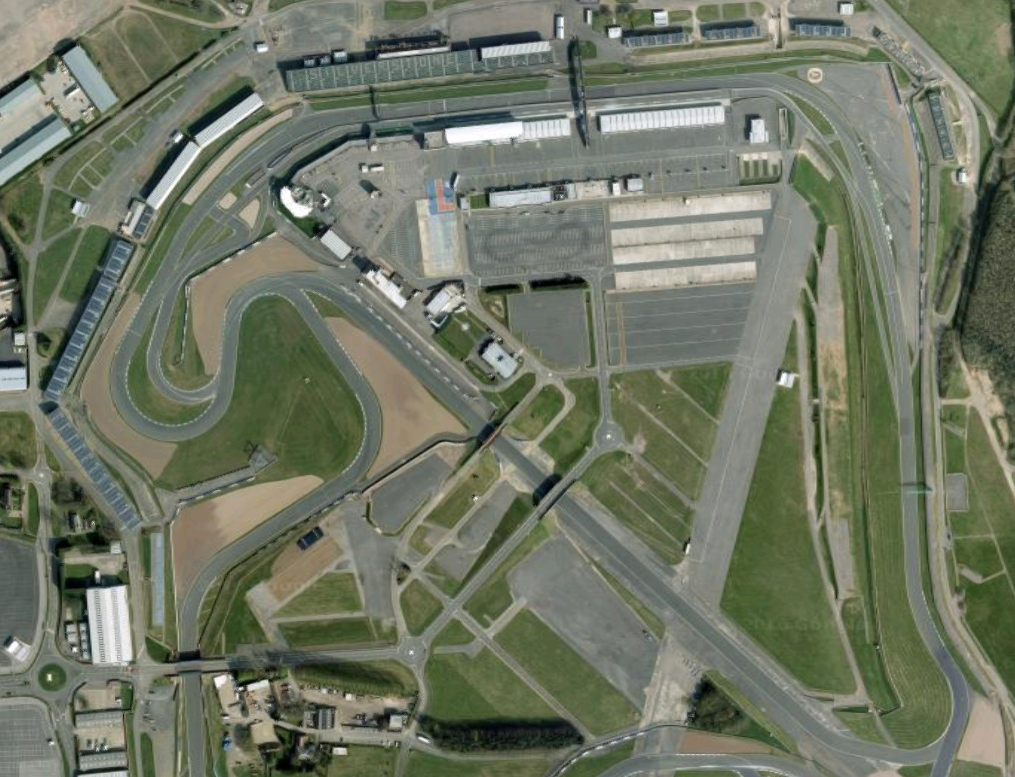
\includegraphics[width=\textwidth]{images/confinedCircuit}
		\caption{Example of confined car racing circuit}
		\label{fig:circuit-overhead}
	\end{minipage}\hfill
	\begin{minipage}{0.45\textwidth}
		\centering
		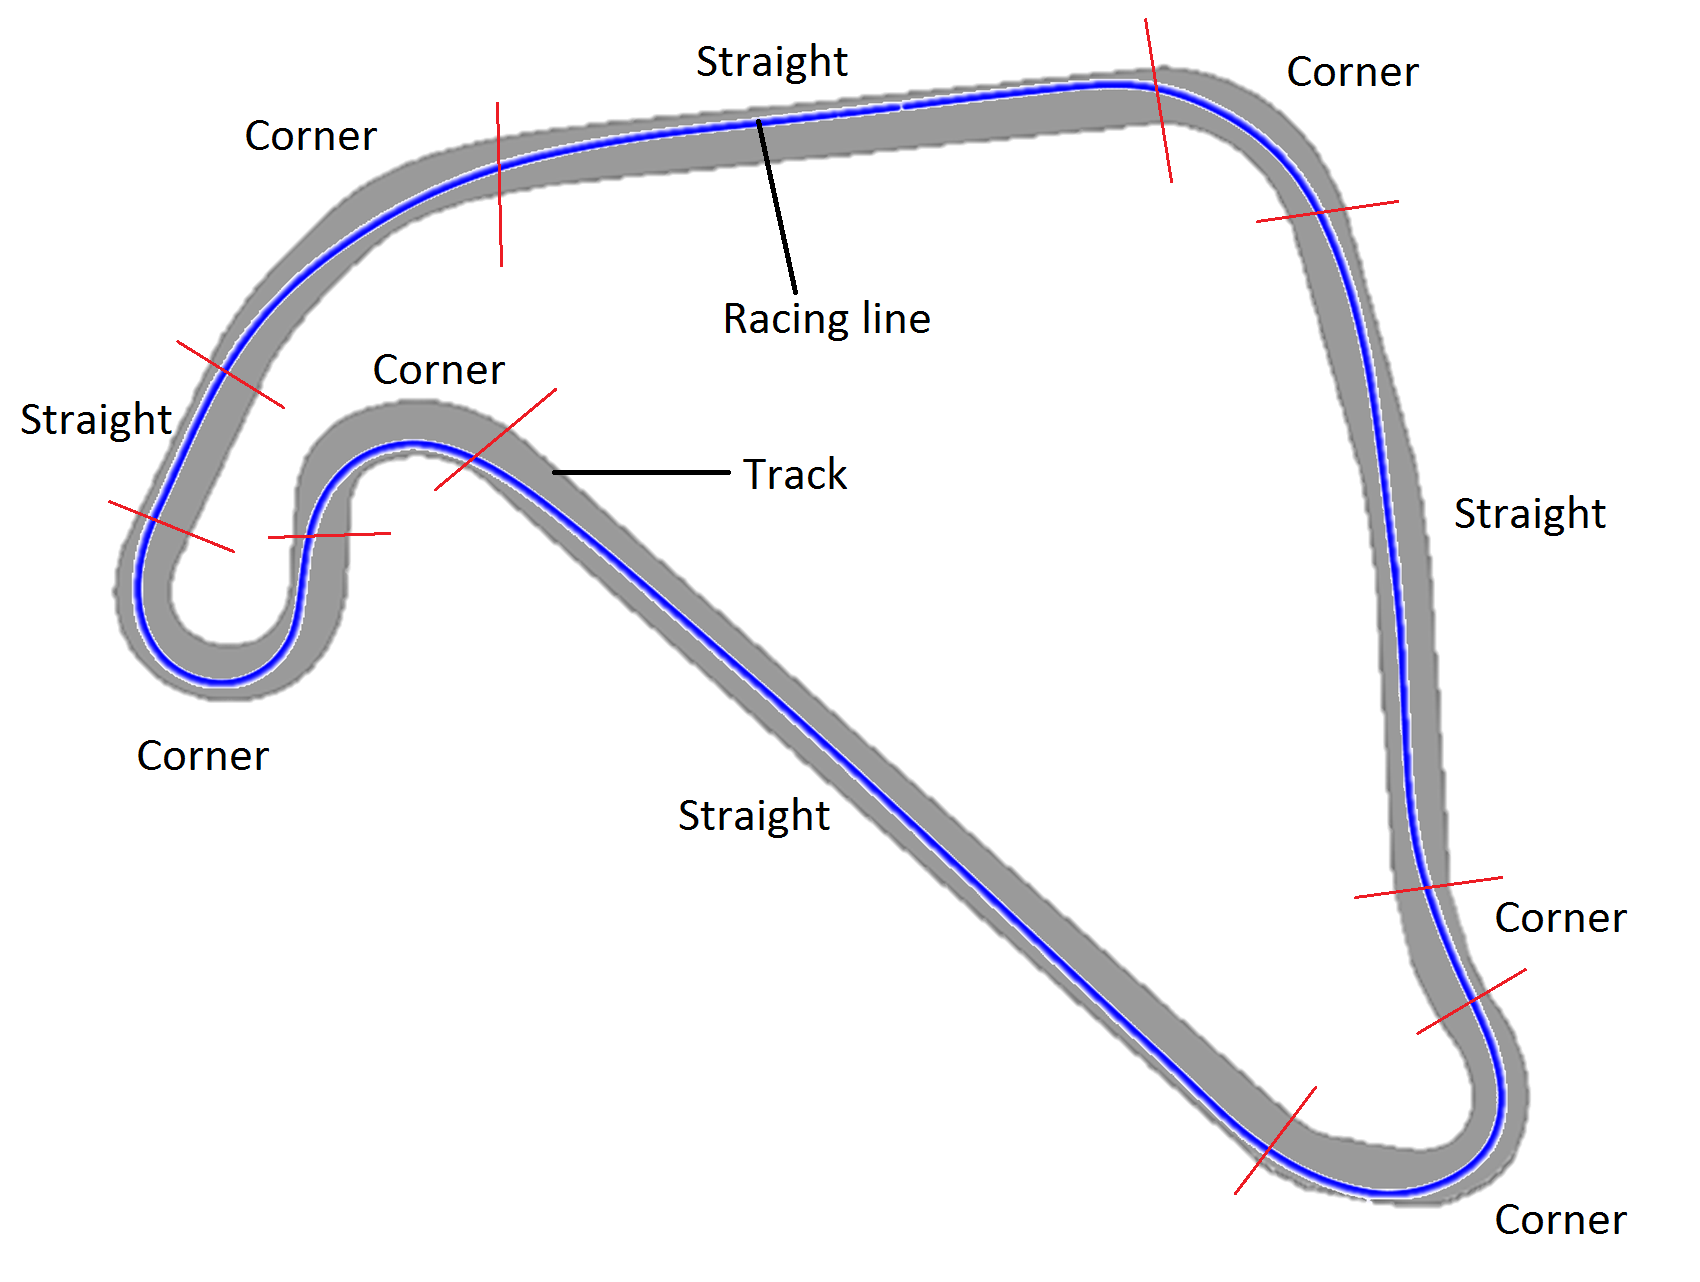
\includegraphics[width=\textwidth]{images/exampleofraceline}
		\caption{Example of racing line, straights and corners}
		\label{fig:circuit-breakdown}
	\end{minipage}
\end{figure}

\begin{figure}[!htb]
	\centering
	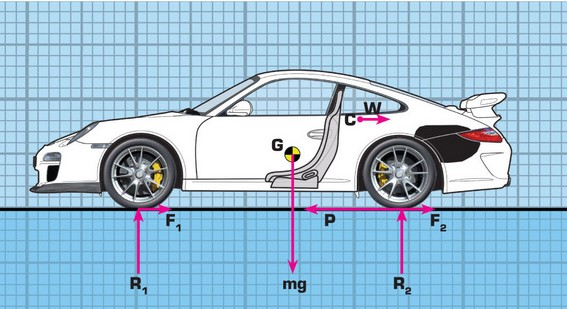
\includegraphics[width=\textwidth]{images/forcesoncar}
	\caption{Forces acting on a car\cite{carscienceForces} }
	\begin{description}
		\item[mg] The car’s weight, which is a force acting at G, the centre of gravity
		\item[R1, R2] Upwards reactions to mg
		\item[F1, F2] Rolling frictional forces acting at the wheels, always in the direction opposing motion.
		\item[P] The engine’s torque, converted to a force P between the rear tyres and the road.	
		\item[W] Drag
	\end{description}
	\label{fig:forces-car}
\end{figure}

\subsection{Racing Line}
\emph{A race driver needs to figure out how to go round a piece of asphalt in the minimum amount of time} \cite{GoingFaster}. In order to do so, he or she needs to develop techniques for more advanced vehicle control. One such technique is that of mastering the racing line (see Figure \ref{fig:circuit-breakdown}), which is considered the fundamental skill a race driver must understand and master before moving on to anything else \cite{GoingFaster}. The racing line is the best path through a circuit: if followed, it is the path that yields the shortest time at the highest average speed \cite{beckman1991physics}. The trickiest part of the racing line to master is that which overlaps circuit corner segments (see Figure \ref{fig:circuit-breakdown}). There are two aspects to mastery of the racing line: first, one has to identifying the path which should be taken, and secondly, one must stay on that path. In the first instance, one has to be able to visualise the racing line, while in the latter one has to control the car such that it stays on the line whilst achieving the highest possible average speed. Once the driver can visualise the racing line, he must further partition it, at and near a corner, in three sections. The first section is the breaking part, where the car needs to sufficiently decelerate in preparation for the corner. Braking is usually carried out in a straight line, ending right before the \emph{turn-in point}. The turn-in point refers to a point on the racing line where steering input is applied, forcing the car to turn into the corner. This action should be carried out smoothly, without jerking motions, taking the car all through the corner without too much correction to the steering. Smooth cornering prevents any abrupt changes to the g-forces and centre of gravity of the car (see Figure \ref{fig:forces-car}), which would result in unpredictable car behaviour \cite{GoingFaster}. Thus, the second partition of the racing line at a corner is the segment between the turn-in point and the apex point, which is the inside mid-point of the corner (see Figure \ref{fig:CornerRaceLine}). After the turn-in point, the driver aims for the apex point. The final section of the racing line in a corner lies from the apex point onwards, where the driver must gradually accelerate out of the corner, while still turning, aiming for the outside apex (see Figure \ref{fig:CornerRaceLine}.

\begin{figure}[!htb]
	\centering
	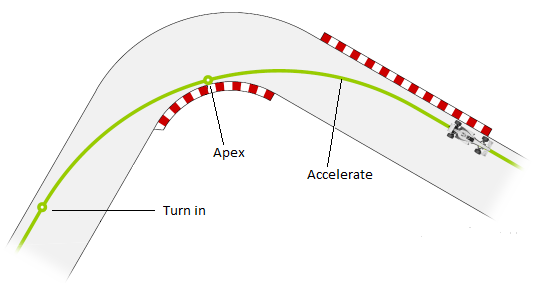
\includegraphics[height=7cm]{images/cornerraceline}
	\caption{Racing line through a 90" right corner}
	\label{fig:CornerRaceLine}
\end{figure}

As the driver gets acquainted to the racing line, usually at sub-optimal speeds, he must find the limit of the car, which is the highest speed the car can be driven while still retaining some measure of control. Various studies have been carried out to define such a limit in terms of the physical properties of the car and its environment \cite{beckman1991physics}. The most important property is the level of grip the car can achieve and sustain on track. A number of factors contribute to the level of grip. Most notably, one very important factor is the tyres as they are the only contact the car makes with the track, and allow for braking, accelerating and turning forces to be transferred to the asphalt. 

Each tyre has two properties which are of particular interest: the slip angle and slip ratio (see Figure \ref{fig:slipangle}). The slip angle is the angle between the tyre's desired direction (perpendicular to the axis of rotation of the tyre) and the tyre's actual direction (the direction the car is moving in). Given both the actual direction of travel ($\mathbf{d}_t$) and the desired direction ($\mathbf{d}_d$) are known, the slip angle $s_a$ is calculated as follows:
\begin{equation}
	s_a = \cos^{-1}(\hat{\mathbf{d}}_d \cdot \hat{\mathbf{d}_t}),
\end{equation}
\noindent where $\hat{\mathbf{d}_d} = \frac{\mathbf{d}_d}{|\mathbf{d}_d|}$ and $\hat{\mathbf{d}_t} = \frac{\mathbf{d}_t}{|\mathbf{d}_t|}$ are the normalised direction vectors for desired and travel directions respectively.

\begin{figure}[!htb]
	\centering
	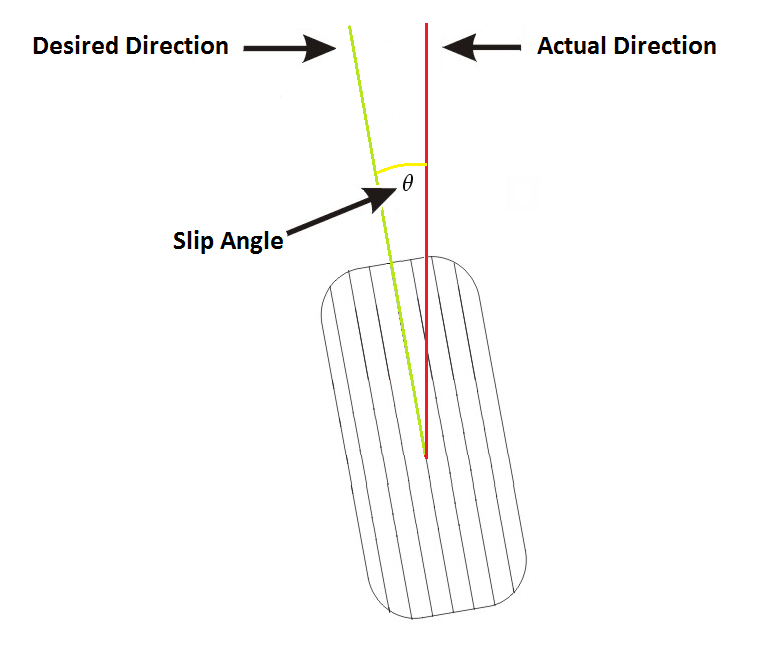
\includegraphics[height=7cm]{images/slipangle}
	\caption{Slip Angle of a tyre understeering while turning left}
	\label{fig:slipangle}
\end{figure}

\subsection{Cornering and Braking}
Whenever the slip angle is above $0\degree$ ($s_a > 0$) the tyre is said to be in an understeering situation. Symptoms include reduced friction, drifting towards the outside of a bend and possible tyre noise from the wheels. Assuming the tyres are not damaged and the track is neither wet nor dirty, understeer can be caused by active factors such as cornering speed, throttle application, braking, steering inputs and weight transfer. Other passive factors such as weight distribution, drive layout, suspension and chassis setup, tyre type, wear and pressures also affect understeer. An understeer situation may be caused by entering the corner at excessive speed, accelerating too aggressively in the corner, breaking through a corner or making sudden input changes which drastically upset the weight distribution of the car. A tyre has an optimal slip angle at which grip is maximised during cornering. The optimal slip angle for a road tyre is about $5\degree$, whereas for a slick tyre, which is purposely constructed for racing, is about $8\degree-10\degree$ \cite{beckman1991physics}.

An oversteering situation may arise from lack of grip; while understeer is caused by a lack of grip in the front tyres, oversteer is cause by a lack of grip on the rear tyres. Oversteer is usually denoted by the rear of the vehicle becoming unstable resulting in its rotation such that the driver is facing towards the inside of the corner. Similarly to understeer, the active factors causing oversteer are also cornering speed, throttle application, braking, steering inputs and weight transfer. Oversteer is usually induced by braking during a corner or accelerating too hard in a rear wheel drive vehicle.

\begin{figure}[!htb]
	\centering
	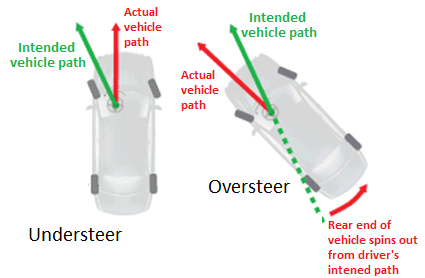
\includegraphics[height=7cm]{images/overundersteer}
	\caption{Visual representation for oversteer and understeer}
	\label{fig:overundersteer}
\end{figure}

During acceleration and braking the tyre experiences rotational forces; when these rotational forces do not match the expected velocity, there is some level of slip occurring between the tyre and the road. This is referred to as \emph{slip ratio} and is expressed as a percentage: a slip percentage of 100\% means that the tyre is rotating but the road is stationary. In jargon, this is called \emph{burnout} or \emph{wheel spin}. On the other hand, a percentage of -100\% indicates that the tyre is not rotating but the road beneath is moving. This can occur when braking too hard and is called \emph{locking the wheels} \cite{pacejka2006tire}. While braking the driver must avoid locking up the tyres as this will cause them to wear out more quickly, while drastically increasing the stopping distance. Conversely, braking too lightly makes the car decelerate at a slower rate, losing the driver precious time. For an optimal braking procedure, the slip ratio should be between 10\% to 15\% \cite{GoingFaster}.

Passive factors, which depend on the mechanical set up of a car, may also influence car behaviour during cornering and braking. However, in this work, any passive factors will be normalised and kept constant across all the study to eliminate any possible effects on dependent variables. 

\subsection{Telemetry Data}
Telemetry (literally remote measurement), is the automated communications process by which measurements and other data are acquired from remote or inaccessible objects or sites, to be subsequently monitored \cite{nasaTelemetry}. Telemetry data is domain specialised data that contains such measurements, transmitted to receiving equipment for remote monitoring. In motorsport, telemetry data contains measurements of vehicle dynamics from the engine and other components. These measurements can serve to monitor and reconstruct the vehicle state at a particular point in time. Telemetry data in motorsports usually accounts for measurements of speed, engine speed, component temperatures, slip angles, slip ratios, etc. Telemetry is widely regarded as the most important source of information by motorsports engineers; analysing this data can lead to a better understanding of the respective strengths and weaknesses of the car and the driver \cite{CarDataAnalysis}. In this work, we posit that through the real-time analysis of telemetry data, the pedagogical aspect of sim racing can be exploited to teach race driving to non experts.  

\begin{figure}[!htb]
	\centering
	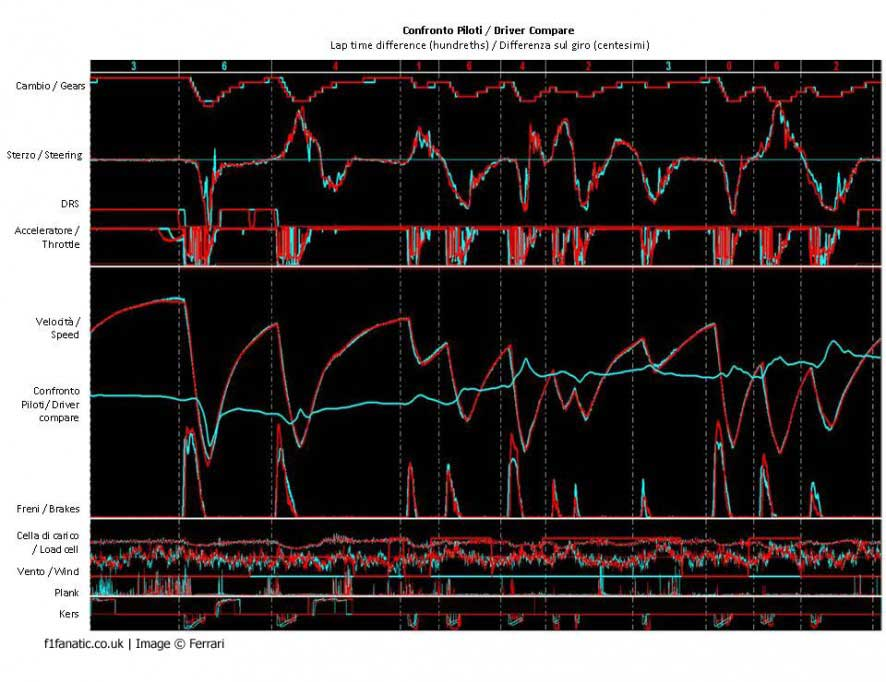
\includegraphics[width=\textwidth]{charts/telemetrydata.jpg}
	\caption{Visualisation of racing car telemetry data}
	\label{fig:telemetrydata}
\end{figure}

\section{Racing Simulation Rigs}
The racing simulation rig (sim racing rig) is a piece of equipment designed to mimic the cockpit of a real-world car (see Figure \ref{fig:racecarcockpit}). The quality of a sim racing rig is dependent on its authenticity - how similar it is to a real-world car - and its build quality. These rigs come in various shapes, forms and sizes, from hangar-sized hydraulic-driven car chassis, that cost millions of Euro, to the more modest, built from off-the-shelf commodity hardware. Minimally, a rig should provide a steering wheel, seating and a display. More sophisticated rigs augment the user experience by employing gear shifters, and clutch, throttle and breaking pedals. The more advanced components are furnished with a force feedback mechanism, a form of haptic technology used to replicate the sense of touch by applying forces or vibrations, or motions to the user \cite{li2015can}. Force feedback may be caused by electrical motors, gear trains or hydraulic systems. In high-end rigs, for instance, hydraulic systems are used to simulate the latitudinal and longitudinal forces to which a driver is exposed during driving. Modern rigs might include virtual reality headsets as a replacement for displays, to enhance immersion and increase realism.

\begin{figure}[!htb]
	\centering
	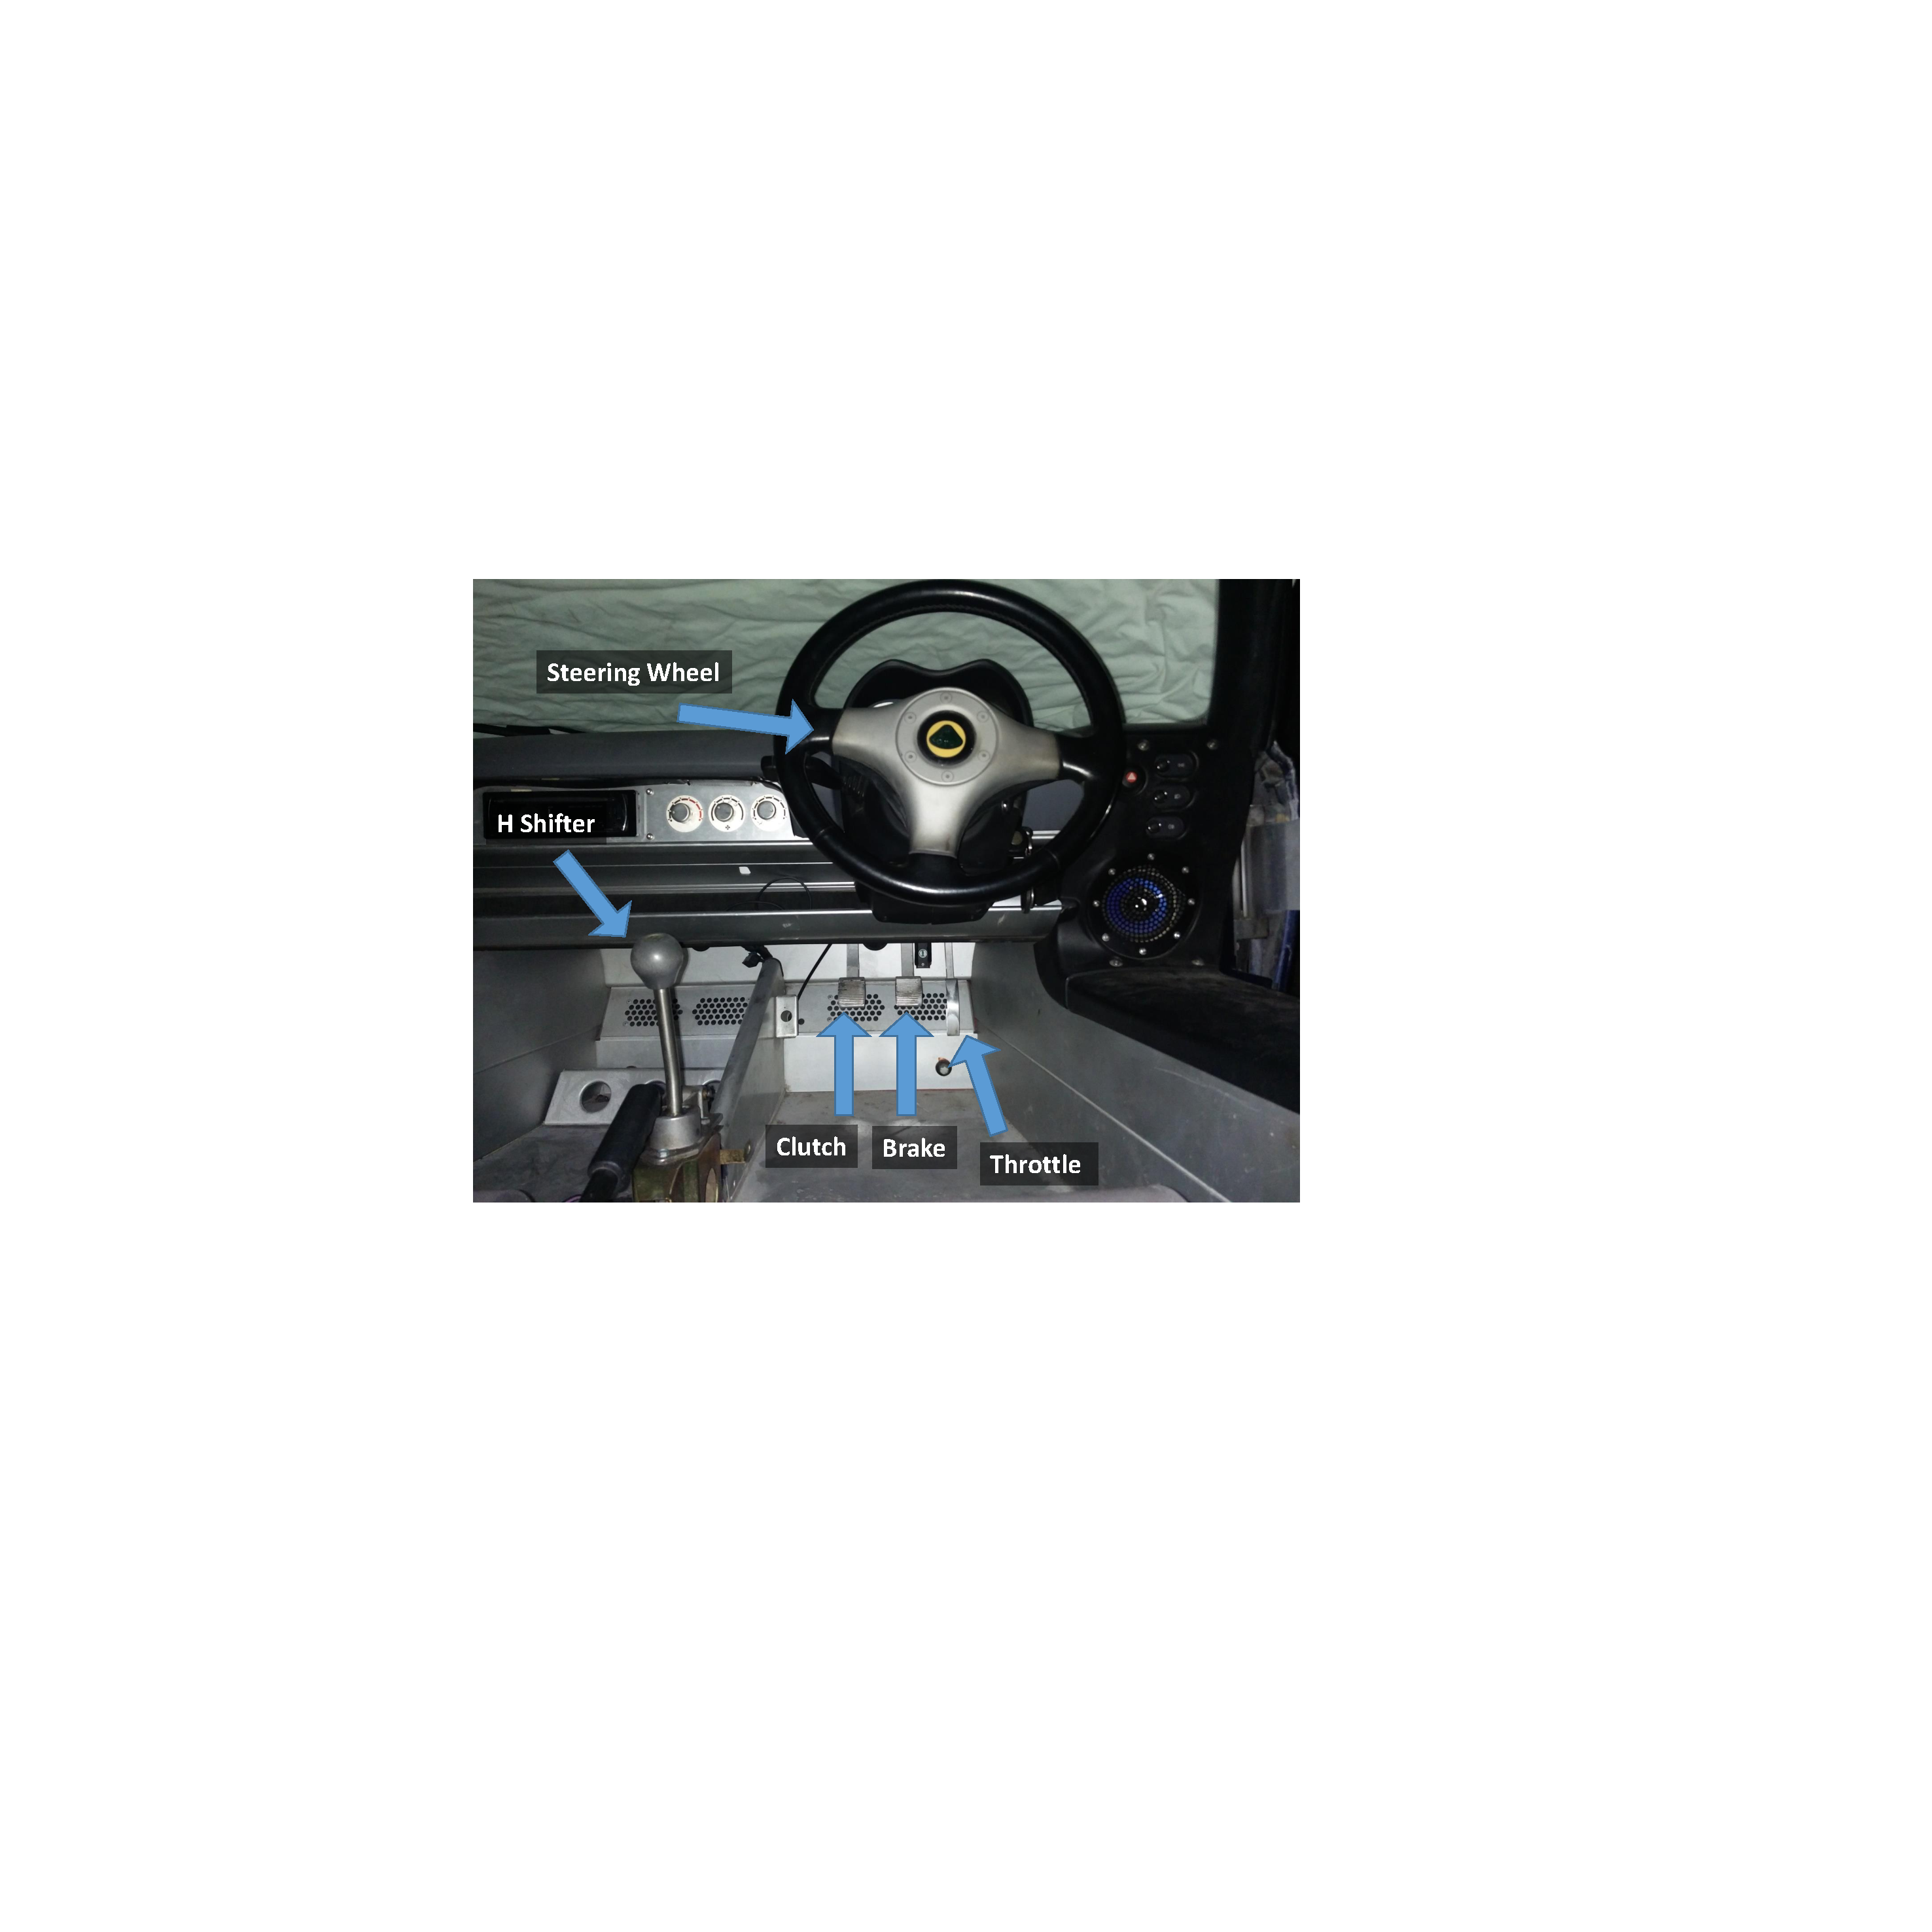
\includegraphics[width=\textwidth]{images/racecarcockpit.pdf}
	\caption{Typical race car cockpit}
	\label{fig:racecarcockpit}
\end{figure}

\begin{figure}
	\centering
	\begin{minipage}{0.45\textwidth}
		\centering
		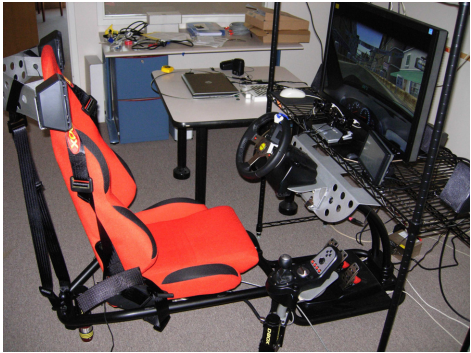
\includegraphics[width=\textwidth]{images/rig1}
		\caption{Entry level racing rig}
		\label{fig:Entrylevelracingrig}
	\end{minipage}\hfill
	\begin{minipage}{0.45\textwidth}
		\centering
		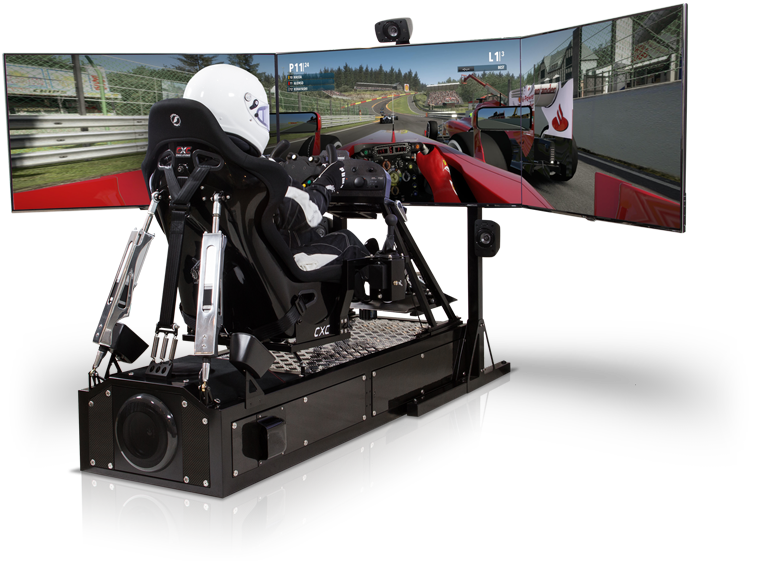
\includegraphics[width=\textwidth]{images/rig2}
		\caption{High end consumer racing rig}
		\label{fig:Highendconsumerracingrig}
	\end{minipage}
		\centering
		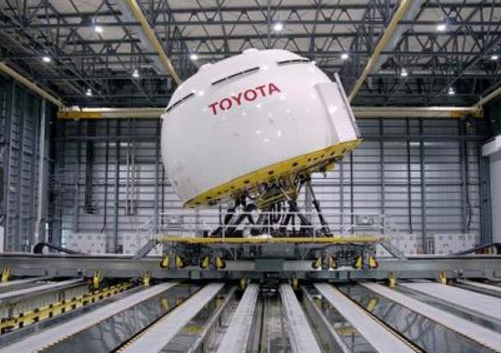
\includegraphics[width=0.45\textwidth]{images/rig3.png}
		\caption{High end commercial racing rig}
		\label{fig:commercialracingrig}
\end{figure}

\section{Summary}
In this chapter motorsport has been introduce and described, further more the ground work for becoming a good race driver has been laid out and finally sim race rigs have been introduced and described. The next chapter will focus more on academic literature which is of interests to this project.

TO ADD - Racing rigs, force feedback, Telemetry data what it is what it contains, Expert Systems

\newpage

\section{Literature Review}

\subsection{Video games and Serious Games}

Baranowski et al \cite{yuserious} define games as a physical or mental contest with a goal or objective, played according to a framework, or rule, that determines what a player can or cannot do inside a game world. The definition covers the setup of a game, while a physical or mental contest, played according to specific rules, with the goal of amusing or rewarding the participant the reward aspect of games.

Video games are built on top of these core values with the addition of having the game world confined to some sort of digital medium. The first video game was created by William Higinbotham; it was a tennis game to be played on a television set\cite{stanton2015brief}. From the early days of video games, their main aim was always to provide some degree of entertainment. The entertainment value is achieved in various ways depending on the gaming platform, game genre and the target audience. Modern video games are simply made up of three fundamental components: story, art and software \cite{zyda2005visual}.

Moving on to serious games this type of games are considered a mix of simulation and game to improve eduction \cite{abt1970}. The idea behind a serious game is to connect a serious purpose to knowledge and technologies from the video game industry\cite{michael2005serious}. The boundaries of serious games are debated, mostly due to the fact that serious games attract multiple domains making it hard to come up with a common boundary. However, the common denominator across all domains seems to be serious game designers use people's interest in video games to capture their attention for a variety of purposes that go beyond pure entertainment\cite{djaouti2011classifying}.

The main contrast between video games and serious games is the use of pedagogic activities which aim to educate or instruct knowledge or skill \cite{zyda2005visual} in serious games as opposed to the pure leisurely aspects of the video game. Pedagogy is given preference over the amusement value which in some cases might not be found in serious games \cite{zyda2005visual}. All serious games involve learning, whether eye hand coordination skills, visual-spatial skills,  which buttons to push or what to do in a certain scenario. This is the fundamental difference between serious and entertainment games. Serious games need to educate the player with a specific type of content, whereas entertainment games need to entertain the player with whatever; racing, puzzles, it does not really matter, as long as the player enjoys it\cite{Harteveld2007}. With an entertainment game, development's main objective is too make the game fun, the content and controls should be at the service of making the game entertaining, On the other hand, serious game designers have multiple objectives, they still need to create a compelling and fun game, but also an educating and realistic game.  From this it follows that three aspects as essential for a serious game, fun, learning and validity \cite{Harteveld2007}. One should not forget that a serious game is fundamentally a game, and a game should be fun. The game should make use of pedagogical methods and theories to ensure knowledge can be conveyed. Validity is related to the content which is being tackled in the serious game. The content which is being taught should teach relevant content that can be applied outside of the game world.

\subsubsection{Pedagogy}
In order to produce a valid pedagogical experience aspects as learning objectives, target groups and challenges needs to be clearly identified before designing a serious game\cite{moser2002methodology}. Various pedagogy theories exist which can be applied to a serious game, some of which are behaviorism, cognitivism, constructivism and situated learning\cite{egenfeldt2005beyond}. From each of these theories one can extract some important properties. 

\begin{description}
\item[Experience] Games tend to provide learning-by-doing, Many games make use of pop-up windows with extensive amount of text that are supposed to have educational value. This technique could provide too much information, time pressure or other factors inside a game environment which could potentially lead to cognitive overload or lead a person to filtering out critical information\cite{egenfeldt2005beyond}.

\item[Exploration] An important property of a game is that of requiring an active, participative attitude of the learner. The game world, including rules, mechanics and environment need to be explored and discovered by the learner. Many poorly designed games force the player to do something, while they should just let the player figure it out or at least guide the player into doing so.

\item[Incremental] The learning process should occur incrementally as it will otherwise be too demanding for a player, and that is the way the human brain functions. Humans acquire knowledge piece for piece and try to integrate this into existing structures\cite{moser2002methodology}.
\end{description}

Deciding on a pedagogy is no easy task, one must take into account the aims and objective which is the pedagogy task is trying to achieve while also considering any capabilities and limitations the target audience might have. Such consideration must be made when designing the way information is channelled back to the user. Three main channels are considered, auditory, visual and kinaesthetic. The choice of which to use relies heavily on the domain and the end user. Some instructions might be able to be better conveyed through visual cues, while other work better as auditory or kinaesthetic, however, previous work found out that a mix of channels work better as one can complement the other\cite{leahy2003auditory}. Such cases include instances in which timing is a factor, having a visual image further explained with audio or vice versa. A further consideration has to be made when applying this to the vehicle driving context, it is important avoid or at least minimise the effect such channels might have on the concentration of the driver. The driver is already focusing by keeping eyes on the road, usually focusing on the centre of the road ahead also keeping in the look out with rapid eye glancing at any obstacles in the vehicle surrounding area and staying attentive for any auditory cues coming from the environment which could highlight any danger\cite{engstrom2005effects}. 

\subsection{Sim Racing}
Simulation racing games (sim racing) such as Asseto Corsa \cite{assestoCorsa} and Project CARS \cite{ProjectCars} , which are off-the-shelf products, provide a sim racing experience within budget for the average video game consumer. The aim with such games is to replicate real life cars, race car dynamics and track locations to amuse and entertain the player. The challenge aspect is achieved by pitting the user against other computer drivers known as AI players, or in multiplayer online races, which are played against other human players. In some cases, a user can compete against oneself by taking on a ghost - a recording of the player's best lap for a particular track. Sim racing the definition of what a video game is however, they miss the pedagogy activities which would qualify them as serious games. Most of the modern sim racing games do aid the player to improve by means of implementing aids. Such aids might include showing the racing line while also highlighting the braking and acceleration points. Other aids include anti lock brakes, traction control and stability control, these are implemented in a passive way. With the exception of the racing line, the player is not told when and what is being done wrong. This results in users having to figure out their own mistakes by means of practicing without any guidance or feedback from with the game. This final year project aims to implement a module which is plugged into an off the shelf racing simulator which. This module trains users by letting them know what is being done wrong, when it's being done wrong and most importantly how to avoid making the same mistake. Further more this project builds on the premise put forward which shows that users are able to learn road driving skills into a virtual world and then successfully applying them to the real world\cite{li2015can}\cite{vogel2006computer}. Although studies have been carried out involving training for road drivers, none have looked into teaching on racing circuits with the aim of improving racing and car handling techniques. 

\newpage

\newpage
\chapter{Research Methodology}
\label{chp:methodology}
This chapter provides a detailed exposition of the methodology used throughout this work. This study has conducted exploratory and descriptive research to determine whether the use of simulation and an automated feedback driven system, a user can be trained as a race driver. The chapter is structured as follows: \S\ref{sec:meth-overview} provides a general overview of the overarching methodology used in the study, \S\ref{sec:meth-experiment-setup} describes in length the design of the instrument used to acquire experiment data and results, \S\ref{sec:meth-experiment-structure} presents the experimental procedure and the rationale behind it, \S\ref{sec:meth-data-gathering} identifies the information and data acquired through the experimental and descriptive methodologies employed, and finally \S\ref{sec:meth-data-analysis} presents the data analysis mechanisms employed to substantiate our conclusions.
%
% Overview
%
\section{Overview}
\label{sec:meth-overview}
This study conducted experimental and descriptive research on the viability of the use of simulators in conjunction with an automated feedback system for improving race driving skills in the normal population. Specifically, a user study was devised and carried out with the primary goals being:
\begin{enumerate}
	\item To determine whether a context-based feedback system can improve the skills of a participant
	\item To quantify the magnitude of this improvement, if (1) is true
\end{enumerate}

These goals were addressed by means of an experimental setup based on a race-driving simulator, using which objective measurement of the participant performance could be gathered and analysed, and a questionnaire for relating the participant's experience with the experimentally-gathered data. The setup of the experiment is explored in more detail in \S~\ref{sec:meth-experiment-setup}.

Since the main goal of this study is that of assessing how effective a feedback system is in the learning process, the independent variable in the experiment is the ability to receive feedback. The hypothesis is that participant performance (such as average lap time) is improved through feedback, and is thus a dependent variable. However, practising without feedback can also lead to changes in the dependent variable; therefore this is controlled for by having two groups of participants: the experimental group that receives feedback and the control group that doesn't. Random assignment is used to determine a participant's group.

A questionnaire, to be administered to the participants at the end of the session, will be designed to help normalise and control for other factors that may influence dependent variables, and hence, the outcome of the experiment. The design of the questionnaire also helps in bridging the participants' perception of their performance with the actual performance data, possibly providing further insight into the results. A questionnaire was preferred to an interview because it is easier to administer, it lends itself to group administration and also allows confidentiality \cite{introductiontobehavioralresearchmethods}.. It is indeed true that interviews permit a greater freedom of expression on behalf of the participant; however, questionnaires create a sense of anonymity that encourages the participants to be more truthful in their answers \cite{introductiontobehavioralresearchmethods}.

\section{Experiment Design}
\label{sec:meth-experiment-design}
In the experiment, each group would be utilising the same car and racetrack. Bastow et al. \cite{bastow2004car} suggest that cars equipped with a front wheel drivetrain may be easier to handle. The Fiat 500 Abarth was the car chosen for the experiments, partially based on Bastow et al.'s findings. The car is relatively low-powered and thus, easier to use by beginning drivers. The Silverstone National race track has the desirable properties of being flat and smooth, without uneven surfaces or bumps which may result in loss of control in rookie drivers. Furthermore, the way the track is structured, with wide run-off areas located along the circuit where drivers are most likely to lose control of the car, allows the car to slow down before colliding with barriers or other stationary objects.

Two feedback mechanisms have been considered for this experiment, \emph{visual}, through the use of a heads-up-display (HUD) superimposed on the simulation display, or \emph{auditory}, by means of descriptive speech projected through loud speakers. Leahy et al. \cite{leahy2003auditory} argue that auditory feedback is less intrusive than visual clues; based on these findings, it was decided that the system should provide feedback using auditory clues.

\begin{figure}
	\centering
	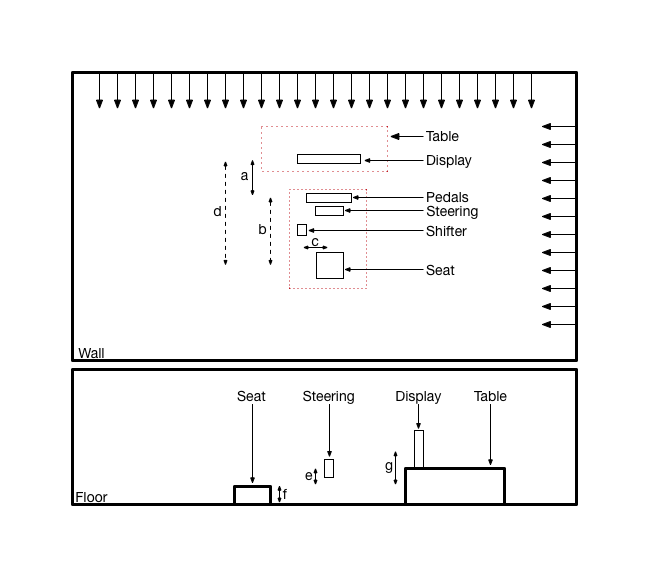
\includegraphics[width=\textwidth]{images/experiment-setup-schematic.png}
	\caption[Experiment Setup Schematic]{Top-down and side views of experiment setup}
	a = 45cm, b = 75cm, c = 36cm, d = 120cm, e = 20cm, f = 30cm, g = 35cm
	\label{fig:meth-experiment-setup}
\end{figure}

\section{Experiment Materials}
\label{sec:meth-experiment-setup}
The setup of the experiment was divided into three material categories: \emph{simulation environment}, \emph{simulation hardware} and \emph{simulation software}, with each category subscribing to a number of desirable properties: 

\begin{description}
	\item [Environment] The experiment should be carried out in an isolated, noise-free and well-lit room. Participants would be let in the room one at a time, to ensure the experiment is conducted without any distractions.
	\item [Hardware] The hardware components identified for this experiment are the (i) display output, (ii) audio output, (iii) steering wheel, (iv) gear shifter, (v) acceleration, brake and clutch pedals and (vi) seating frame.
	\begin{description}
		\item [Display and Audio] A 32"+ display capable of outputting graphics at a progressive resolution of 1080 pixels vertically at 60 Hz (1080p60) is required; smaller display sizes would not yield a large enough solid angle for the participant to feel immersed in the simulator. For audio output, a stereo setup with a speaker output power of 10W should be sufficient; at a distance of 1m, these speakers can generate sound volume up to 100db, where normal conversation is around 60db.
		\item [Driving Controls] The driving controls include (ii)-(iv); minimally a steering wheel should provide the same number of revolutions as a racing car, providing accurate force feedback to let the participants accurately assess the behaviour of the car. Gear shifters do not implement feedback mechanisms; however, given their ubiquity, H-shifters are preferred since they are the kind most drivers are familiar with. High-end pedal systems use hydraulics to simulate the variability of force required on part of the driver to actuate a pedal during different stages.
		\item [Seating Frame] The seating frame should ensure a seating position akin to a driver in a racing car. The seating frame should also provide the ability to move the seat back and forward in order for participants to be able to seat comfortable and be able to reach the pedals.
	\end{description}
	\item [Software] The software aspect of the experiment, which is primarily the racing simulator, should have a number of desirable properties. In particular, the simulator should provide (i) a realistic driving model, (ii) driving aid customisation, (iii) high-fidelity graphics, (iv) real-world tarmac circuits, (v) and telemetry data access through an interface that is intuitive to use.
	\begin{description}
		\item [Realistic Driving Model] For this experiment, a realistic driving model is a sine qua non. Recreating real-world conditions requires a high-fidelity physics simulation of race car dynamics that is as close to the real thing as possible.
		\item [Driving Aid Customisation] Required to control experiment variables, such as tyre wear and tear. The aim is to prevent car behaviour from changing as the experiment progresses. 
		\item [High-fidelity Graphics] Required to provide the participant with a fully immersive experience.
		\item [Real-world Tarmac Circuits] Most racing simulators accurately replicate real-world tracks, up to minute details such as elevation changes and bumps. This level of realism exposes participants to real-life scenarios. Furthermore, the simulator should provide circuits that loop, to streamline experiments and remove the need to reset the software in order to drive another lap.  
		\item [Telemetry Data Access] The premise of this project hinges on the ability to read telemetry data from a simulator. Thus, any software that does not provide this feature is a priori discarded. However, easier and cleaner interfaces for reading telemetry data, and the breadth of telemetry data offered, are a deciding factor in the choice of racing simulator to use.
	\end{description}
\end{description}

\subsection{Hardware Selection}
A number of racing simulator input devices have been considered (see Table \ref{tab:racing-input}). The choice was narrowed down to the most popular devices among racing game enthusiasts, the Logitech G25~\cite{logitecg25}, the Thrustmaster TX~\cite{TrustmasterTX} and the Fanatec CS~\cite{Fanatec}. The G25 provides the minimally required features: a steering wheel with a $900\degree$ turn, 3-pedal set, H-shifter and force feedback; furthermore, the G25 is also a very affordable device. Both the Thrustmaster and Fanatec are high-end devices, which explains the cost difference. Furthermore, neither come with the 3-pedal set and the H shifter, which have to be purchased separately. The Logitech G25 was chosen for being the most cost-effective of the three options.

\begin{table}[htb!]
    \centering
    \begin{tabular}{lccccc}
        \toprule
        \textbf{Device} & \textbf{$900\degree$} & \textbf{3-Pedal Set} & \textbf{H-Shifter} & \textbf{Feedback} & \textbf{Cost} \\
        \midrule
        Logitech G25 & \checkmark & \checkmark & \checkmark & Low & 240 \\
        Thrustmaster TX & \checkmark & & & Med & 324 \\
        Fanatec CS & \checkmark & & & High & 850 \\
		\bottomrule		
	\end{tabular}
	\caption{Comparison of input devices}
	\label{tab:racing-input}	
\end{table}

\subsection{Software selection}
Similarly to the hardware selection process, a number of racing simulators have been considered (see Table \ref{tab:sim-choice}). Although there is a myriad of racing simulators available, the selection process narrowed them down to a popular handful: Forza Motorsports 6 \cite{forza} by Turn 10 Studios, Project Cars\cite{ProjectCars} by Slightly Mad Studios, Assetto Corsa\cite{assestoCorsa} by Kunos Simulazioni, iRacing\cite{iRacing} by iRacing.com Motorsports Simulations and Dirt \cite{dirtgame} by Codemasters. Unfortunately, notwithstanding its quality, Forza Motorsports 6 does not provide access to telemetry information. Dirt also suffers from the same shortcoming, in addition to providing very little in terms of track applicability: very few tracks are circuit-based. iRacing provides most of the functionality required by the experiment, however in terms of visual quality it suffers when compared to Project Cars and Assetto Corsa. Finally, the choice between Assetto Corsa and Project Cars was made on the basis of ease of interfacing for the acquisition of telemetry data; here we felt Assetto Corsa provided a clean, intuitive and ultimately superior interface to telemetry acquistion via User Datagram Protocol (UDP) connections.

%The comparison table shows the desired properties a sim game must have, and a selection of games which have been considered. From the start it is clear, Dirt and Forza 6 should be discarded as none provide telemetry data to be read. Assetto Corsa, Project Cars and iRacing are closely matched, however Assetto Corsa has the leading edge as it provides an easy way to interface via UDP, well document and wide developer community who can help. Furthermore Assetto Corsa provides good visual graphics. For these reasons Assetto Corsa has been picked as the sim to be used.

\begin{table}[htb!]
    \centering
    \begin{tabular}{lcccccc}
        \toprule
        \textbf{Simulator} & 
        \multicolumn{1}{p{1.2cm}}{\centering \textbf{Driving} \\ \textbf{Model}} &
        \multicolumn{1}{p{1.2cm}}{\centering \textbf{Driving} \\ \textbf{Aids}} &
        \multicolumn{1}{p{1.2cm}}{\centering \textbf{Visual} \\ \textbf{Quality}} &
        \multicolumn{1}{p{1.1cm}}{\centering \textbf{Tracks}} &
        \multicolumn{1}{p{1.1cm}}{\centering \textbf{Tele-metry}} &
        \multicolumn{1}{p{1.1cm}}{\centering \textbf{I/F Ease}} \\
        \midrule
        Forza & \checkmark & \checkmark & \checkmark & \checkmark & & \\ 
        Project Cars & \checkmark & \checkmark & \checkmark & \checkmark & \checkmark & \\ 
        Assetto Corsa & \checkmark & \checkmark & \checkmark & \checkmark & \checkmark & \checkmark \\ 
        iRacing & \checkmark & \checkmark & & \checkmark & \checkmark & \checkmark \\ 
        Dirt & \checkmark & \checkmark & \checkmark & & & \\ 
		\bottomrule		
	\end{tabular}
	\caption[Comparison of Racing Simulators]{Comparison of racing simulators on the basis of a realistic driving model, customisable driving aids, high-fidelity graphics quality, applicability of tracks, availability of telemetry information, and ease of interfacing.}
	\label{tab:sim-choice}	
\end{table}

%
%\begin{center}
%	\begin{tabular}{ | l | l | l | l | l | l |}
%		\hline
%			& Assetto Corsa\cite{assestoCorsa} & pCars \cite{ProjectCars} & iRacing \cite{iRacing} & Dirt \cite{dirtgame} & Forza 6 \cite{forza} \\ \hline
%		Realistic model	& \checkmark &\checkmark & \checkmark & \checkmark & \checkmark \\ \hline
%		Tracks	& \checkmark &\checkmark & \checkmark &  & \checkmark \\ \hline
%		Disable wear & \checkmark & \checkmark & \checkmark & \checkmark & \checkmark \\ \hline
%		Telemetry data	& \checkmark & \checkmark & \checkmark &  &  \\ \hline
%		Ease of Interfacing	& \checkmark &  & \checkmark &  &  \\ \hline
%		Quality of graphics & \checkmark & \checkmark &  & \checkmark & \checkmark \\ \hline
%	\end{tabular}
%\end{center}

\subsection{Participant Information and Feedback}
Questionnaires are a very important tool for acquiring insight from the point of view of experiment participants, and when compared to interviews, they provide a framework within which respondents can answer more truthfully due to lack of social external pressures. Leary et al. \cite{introductiontobehavioralresearchmethods} provide a set of guidelines for compiling questionnaires, consisting of seven general rules:
\begin{enumerate}
	\item Be specific and precise in phrasing the questions;
	\item Write the questions as simply as possible, avoiding difficult words, unnecessary jargon, and cumbersome phrases;
	\item Avoid making unwarranted assumptions about the respondents;
	\item Conditional information should precede the key idea of the question;
	\item Do not use double-barrelled questions;
	\item Pretest the questions.
\end{enumerate}
Responses from questionnaires designed using these guidelines are valid in the general case. A further challenge posed by questionnaire compilation is that of choosing a response format for each question: open-ended questions may serve to collect more information but be less conducive to analysis, while on the other hand, more restrictive and constrained response formats may lack expressivity but be easier to analyse. Leary et al. suggest using constrained response formats, such as the Likert scale \cite{likert1932technique}, when dealing with behaviours, thoughts or feelings that can vary in frequency or intensity, and open-ended questions in cases where further insight is desired. 

Two qualitative questionnaires have been designed in accord with these guidelines, one with the aim of gathering insight into the participant demographics, and a second to help normalise and control for factors that may influence dependent variables, to bridge the participants' perception of their performance with the actual execution, and to gather other insight and feedback about the experiment.

%A questionnaire, to be administered to the participants at the end of the session, will be designed to help normalise and control for other factors that may influence dependent variables, and hence, the outcome of the experiment. The design of the questionnaire also helps in bridging the participants' perception of their performance with the actual performance data, possibly providing further insight into the results.

%The challenge in choosing a response format in a question lies in identifying whether one should go for an open ended question in which more information might be collected, or on the other hand, use a rating scale response format, where the response is more constrained but may be easier to analyse. Leary et al. suggest using the former for questions dealing with behaviours, thoughts, or feelings that can vary in frequency or intensity (e.g. the Likert Scale\cite{likert1932technique}) and using open ended questions in cases where further insight is desired.

%Based on these guidelines two qualitative questionnaires have been designed, one aiming to gather insight into the sample demographic, the other aiming to gain insight into the participants' impressions about the realism of the experiment setup, the level of comfort, or discomfort and any suggestions or comments they might have. 

%\subsection{Participant Demographic}
%
%\subsection{Participant Feedback}

\section{Experiment Procedure}
\label{sec:meth-experiment-structure}
In this section, we describe in detail the experiment procedure. Participants are gathered through various methods, ranging from word-of-mouth to mailing lists, where each participant would reserve an experiment time slot. Participants are split randomly into two groups. The first group is referred to as the \emph{feedback group}, the second as the \emph{control group}. 

%In order to evaluate the effectiveness of the system a user study took place. Participants were split randomly into two groups. One group will be referred as the feedback group, the other will be referred to as the base group. The experiments structure was subdivided into smaller systemic tasks.

\begin{description}
	\item[Introduction] Each participant is introduced to the setup and given an overview of the experiment procedure. 

	\item[Demographic Questionnaire] The experiment starts by the participant responding to a brief questionnaire, aimed to gather more insight about the general participant demographics.
	
	\item[Rig Configuration] 
	The user climbs inside the rig; the seating position is adjusted to accommodate the user, making sure he or she is sitting comfortably, and all controls can be reached with ease. Participants are given a second, more in-depth overview of the components of the rig and how they operate. This explanation covers the steering wheel, the pedal layout and function and the H-shifter.
	
	\item[Practice (10 minutes)] The participant is given ten minutes to get used to the rig setup, track and car. This session is aimed at gauging the skill level of the user while he or she gets acquainted with the simulator.
	
	\item[Break (5 minutes)] A short break (5 minutes maximum) is given to each participant.
	
	\item[$1^{st}$ Session (10 minutes)] In this session, the participant drives the racing car around the track for ten minutes. Participants in the feedback group have the feedback system turned on, while for the control group, this is turned off.
	
	\item[Break (5 minutes)] A short break (5 minutes maximum) is given to each participant.

	\item[$2^{nd}$ Session (10 minutes)] A second ten minute session is held; participants in the feedback group have the feedback system turned on, while for the control group, this is turned off.
	
	\item[Break (5 minutes)] A short break (5 minutes maximum) is given to each participant.
	
	\item[$3^{rd}$ Session (5 minutes)] A final five minute driving session; the feedback system is turned off for participants in both groups. This session was included to help identifying conclusive results about the feedback system and its effects on the participants. 
	
%	\item[Five minuties session] A final five minuties of driving are allocated yet again, this time with the feedback system turned of for both groups. This was designed to possibly identify any conclusive results. Such session could show the possibility of the feedback group performing worst after having the aid of the feedback system removed or both groups ending up performing the same after the sessions, which would suggest the feedback participant didn't manage to get any cognitive advantage.
	
	\item[Feedback Questionnaire] The experiment concludes by the participant responding to a questionnaire about experiment structure, apparatus quality, performance perception and free-form participant feedback.
	
%	\item[Particpant's feedback questionare] The final stage of the experiment requires participants to fill in the a questionnaire  in which they are asked to give their feedback on the experiment structure, hardware used and any further comments they would like to add.
	
\end{description}

\section{Data Collection and Sampling}
\label{sec:meth-data-gathering}
The data collected during the experiments consists of two questionnaires per participant and four batches of telemetry data per participant. Each batch represents the telemetry data collected in a particular driving session. Google Forms was used to host the questionnaires due to its ease of use and the ability to export data and generate descriptive statistics on that data, such as frequency counts, etc.  

%At the end of the experiments the data collected includes two questioners from each participant and four batches of telemetry data, one for each participant. Questioners are filled online using Google Forms as it provides the ability to export the data and also automatic generation of descriptive statistic. The data collected from the questionnaires and telemetry data is to be loaded into a data base management system from which the data can be queried using specialised data querying constructs. By having a querying language, it provides the flexibility of extracting data which is relevant for the data analysis at hand.

\section{Data Analysis}
\label{sec:meth-data-analysis}
In order to evaluate the performance of each of the two groups (control and feedback) and perform meaningful statistical comparisons between them, the collected data were subjected to Independent T-Test\cite{student1908probable} and the Mann-Whitney U Test\cite{mann1947test}. These are appropriate tests for independent groups \cite{de2015statsref}. In our case, the groups are indeed independent because a participant from the control group may not make part of the feedback group and vice versa. The null hypothesis is that there is no significant difference across the groups, while the alternative hypothesis is that there is significant difference across the groups. The tests are described below:

%In order to accept or reject the null hypothesis statistical test are to be carried out. Most important is the ability to compare the performance of the two groups across sessions. The lap time is used as the test variable as this gives a good indication for the average performance achieved during a lap. Furthermore which comparison test to use depends on the sample size, the distribution of data and the types of group. In this case the groups are independent from each other, as a participant may not be part of the base group and also part of the feedback group. As pointed out by De Smith in his book "Statistical Analysis Handbook-a web-based statistics" the tests of interest to this project are the Independent samples t-test\cite{de2015statsref} and the Mann Whitney U test\cite{de2015statsref} as these test for difference between independent groups. Both tests share the same hypothesis listed below.

\begin{description}
	\item[Independent T Test] This test determines whether there is a statistically significant difference between the means in two unrelated groups. This test assumes the data is normally-distributed; this is verified by testing each group for normality using the Shapiro-Wilk\cite{shapiro1965analysis} test.
	
%	assumes the data is normally as such the data must be checked for normal distribution. This can be carried out by using the Shapiro-Wilk\cite{de2015statsref} test for normality on both groups.
%	
	\item[Mann-Whitney U test] This test does not require the data to be normally distributed; it does, however, assume that the data in the groups share the same distribution. This is verified by using the Kolmogorov-Smirnov \cite{kolmogorov1933sulla} test.
	
%	Does not require the data to be normally distributed however, it assumes the groups' data shares the same distribution. The groups are checked for equal distribution using the Independent Samples Kolmogorow-Smimov \cite{xxx} test.
\end{description}
	
%	\item[Null hypotesis]there is no significant difference across the groups
%	\item[Alternative hypotesis]there is significant difference across the groups
%\end{description}

%As the data distribution is not known before hand, distribution tests will be carried out after the data is collected and depending on the result, the adequate test will be used.

\section{Summary}

\newpage
\section{Specification and design}

The purpose of this section is to give the reader a clear picture of the system/artifact/project/work that has been created in the FYP and why it has been created in the way chosen. 
Details:
• Fine details, specifically details of the system (software or hardware) should be left out. Also, any complete rigorous specification is better relegated to an appendix.
• Using diagrams (including but not limited to flowcharts and system level block diagrams) is strongly recommended.
• Any design choices have to be justified (e.g. by discussing the implications of different design choices and then giving reasons for making the choices made).
• The design of the project will almost certainly have evolved during development. Focus should be made on the project as it is in its final state but often there are good reasons for describing intermediate states too (e.g. to discuss details of the design method used). 

*************************
Hardware

Steering wheel, pedals and shifter
Rig and seat
Displays and sound output
PC

*************************
*************************

Software

Supporting Apps, Track data Editing tool, TTS, 

Spatiasl query complexity

Feedback system workings, how will it determine the algorithm 

Software Project Structure
	IPC
	Input
	Common Shared Layer
	Output
	Pluggable modules


Racing game
	Assetto corsa
	Other games which where considered

*************************

\newpage
\def \methodname {TeAR\xspace}
\def \methodnamefull {Telemetry Assisted Racing\xspace}

\chapter{Design and Implementation}
This chapter provides a detailed description of the design and implementation of the software artefact employed in this project. The chapter starts by giving an overview of the core requirements for the main software artefact which we refer to as \emph{\methodnamefull (\methodname)} (see Section \S\ref{sec:imp-requirements}). Section \S\ref{sec:imp-supportingTools} discusses the tools developed to create content for the feedback system, including track annotation and racing line visualisation amongst others \S\ref{sec:imp-supportingTools}. The chapter concludes with an in-depth description of the internals of the feedback system, the respective components, their integration and communication \ref{sec:imp-systemArchitecture}.

\section{Requirements}
\label{sec:imp-requirements}
Deliberation on the methodologies provided in Chapter \ref{chp:methodology} led to a number of requirements being identified for the software artefact. These requirements are listed below:

\begin{itemize}
	\item Content creation and annotation 
	\item Interfacing with third-party racing sim software 
	\item Efficiently read and process incoming telemetry stream
	\begin{itemize}
		\item Filter the stream for noise and unnecessary detail
		\item Structure raw data to facilitate further processing
	\end{itemize}
	\item Develop a heuristic-based system to provide feedback
	\item Provide a mechanism for communicating feedback to user
	\item Persist telemetry data for further processing
\end{itemize}

Circuit information coming from third-party software, such as the racing line, must be available to \methodname; furthermore, this data is to be annotated with additional information such as track section partitioning and the respective properties, which are fundamental in determining which feedback to provide to the user. Thus, a number of supporting tools have to be developed.
\methodname must interface with the third party racing simulation software (Assetto Corsa) via the inter-process communication system provided by the program. In addition, \methodname must extract a stream of telemetry data from the simulator, at a sampling rate of approximately 333Hz (which is the sustained rate provided by Assetto Corsa).
The incoming telemetry data must be filtered since not all data is useful to \methodname. Furthermore, these data are organised into structures that are more conducive to processing later on in the pipeline. 
This telemetry information will be fed into a heuristic-based algorithm that should return feedback that will eventually be presented to the user. This feedback should be the most effective correction the user would need to make to improve that particular race track section.
\methodname should communicate this feedback to the user via an auditory messaging system. 
Finally, all telemetry data should be persisted onto secondary storage for offline analysis. 

%The following core requirements have been identified for \methodname:
%\begin{description}
%	\item[Abstract Input/Output Interface] The telemetry data input and feedback output needs to be abstracted. Techniclay this does not effect the feedback's effectiveness or accuracy but it is usefull as to be able to change the sim racing game and the type of feedback which is given with out having to change any of the internal components. This allows for fast prototyping especially with the output interface in which one can develop another way to convey the feedback. 
%	\item[Perform Spatial Querying] The feedback system relies on being able to determine the location of the car on track. This is used to determine if the car is in a straight section or corner section, how far away from the race line the car is and if the mid point of the corner is being driven on. 
%	\item[Store telemetry files] In order for the evaluation chapter to be carried out, the telemetry data is required to be stored for later data analysis. This is achieved by writing the telemetry data to a log file which is later uploaded to the database.
%	\item[Query log files]
%\end{description}

\section{Content Creation and Annotation}
\label{sec:content-creation}
The telemetry data stream read-out from Assetto Corsa does not provide sufficient information about the environment for \methodname to make informed decisions about possible feedback. The feedback mechanism used in \methodname is highly dependent on the racing line, which in turn, is a function of the track geometry; however, it is not possible to acquire any meaningful information about the racing track from telemetry data alone. These factors prompted the creation of the \emph{Track Splicer and Visualiser}, a supporting tool that extracts track information from the Assetto Corsa data files and provides additional annotations to this data as required by \methodname. 

\subsection{Track Splicing}
\label{sec:imp-trackSplicer}
The track splicing tool extracts track and racing line information from Assetto Corsa, partitions the data into a number of sections that are annotated as either straight or corner, and finally finds the apex of each corner section. The tool also provides visualisation of the results in case the user needs to tweak the generation parameters. This process is shown in Figure \ref{fig:diagram-trackspliceinputoutput}.

%The track splicer tool has been developed to aid the feedback system's track meta data file creation. It automates the following tasks. Given a series of two dimensional cartesian coordinate denoting a track race line, (i) split the race line into straights and corners (ii) find the mid point of a corner which is used as the apex point and (iii) give a visual representation of the race line, straights and corners. 

\begin{figure}[!htb]
	\centering
	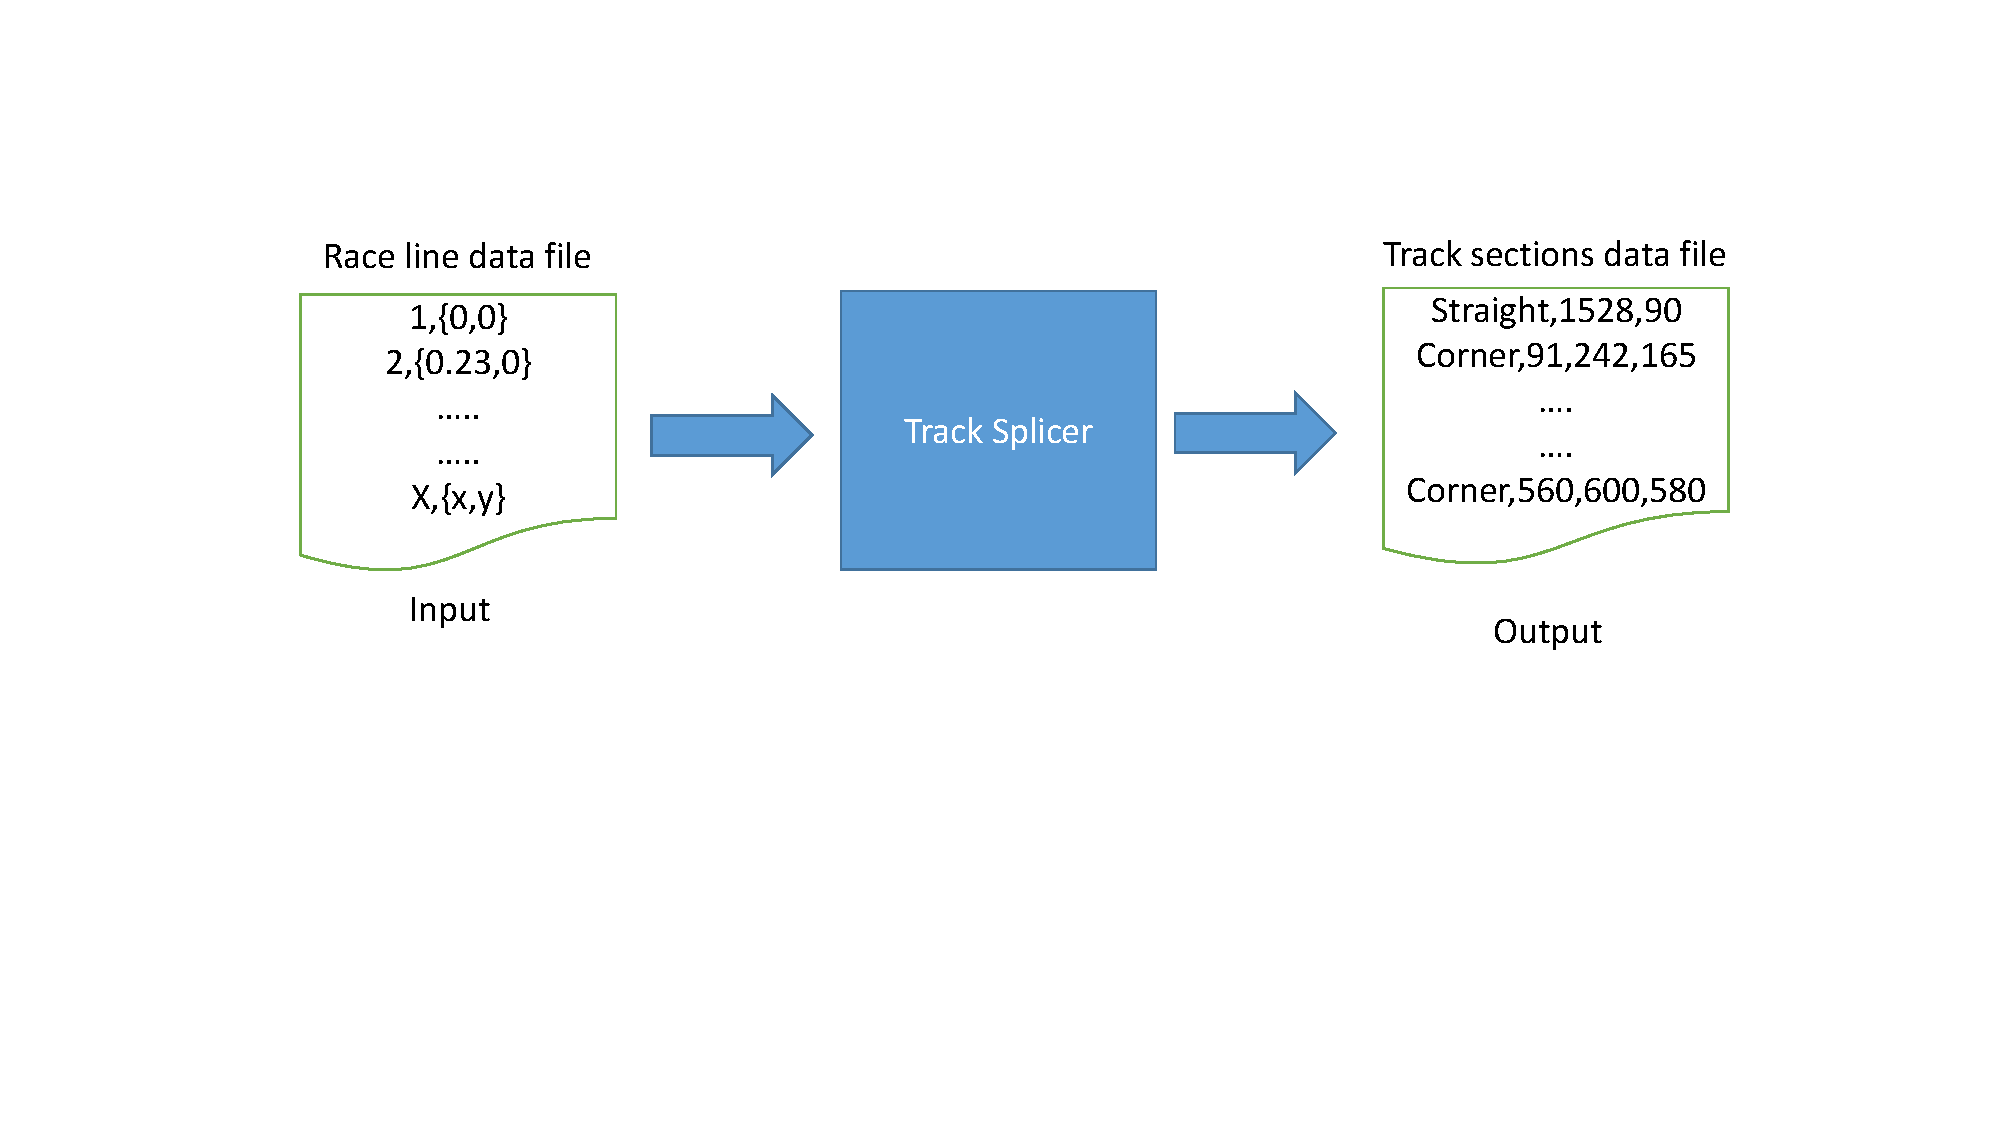
\includegraphics[width=\textwidth]{diagrams/trackspliceinputoutput.pdf}
	\caption[track splicer input out]{Track splicer input and output}
	\label{fig:diagram-trackspliceinputoutput}
\end{figure}

\begin{description}
	\item [Track Partitioning and Annotation] The idealised racing line is a simple closed curve $\mathcal{C}$ on a plane; its digital counterpart is a discrete simple closed curve $\mathcal{C}_d$ with a finite number of vertices, each lying on the curve $\mathcal{C}$ and connected by straight edges - an inscribed polygon - where each vertex $\mathbf{v}_i \in \mathcal{C}_d$ represents a coordinate pair $(x,z)$. The ground is assumed to be a horizontal plane. 	To determine whether a section of the track near a vertex $\mathbf{v}_j \in \mathcal{C}_d$ is a straight or a corner, two further vertices are sampled $\mathbf{v}_i, \mathbf{v}_k \in \mathcal{C}_d$, where $i < j < k \in \mathbb{Z}/|\mathcal{C}_d|\mathbb{Z}$. We define the measure of curvature $c_j$ for the curve at $\mathbf{v}_j$ as follows:
	\begin{equation}
		c_j = \cos^{-1} \left(\frac{\mathbf{v}_k - \mathbf{v}_j}{|\mathbf{v}_k - \mathbf{v}_j|} \cdot \frac{\mathbf{v}_j - \mathbf{v}_i}{|\mathbf{v}_j - \mathbf{v}_i|} \right),
	\end{equation}
	where $c_j$ is the angle between the two normalised unit vectors formed by the ordered vertices $\mathbf{v}_i$ through $\mathbf{v}_k$. A threshold value $c_t$ determines whether the curve segment from $\mathbf{v}_i$ through $\mathbf{v}_k$ is a corner or a straight. A typical value for $c_t$ is 0.5. Edges between consecutive vertices in $\mathbf{C}_d$ may vary in length; therefore, when vertices $\mathbf{v}_i$ and $\mathbf{v}_j$ are chosen, Poisson-Disc sampling is employed, to guarantee that the vertices are no closer to each other than a specified minimum distance $c_m$ (a typical value for $c_m$ is 5).  	

%	\item [Split the race line into straights and corners] This is done by calculating the rate of change of the line by means of vectors dot products. A cartesian coordinate p[x] as 'p1' is considered where x is the position in the array. Two other points are required p[x+1] as 'p2' and p[x+2] as 'p3'. When x is the end of the list, the first two points are used from the list. Using p1, p2 and p3, two vectors are generated, 'v1' which is a vector going from p1 to p2, and 'v2' which is a vector going from p2 to p3. The vectors are normalised as the their magnitude is irrelevant for this computation. The dot product of v1 and v2 is computed, the result is passed through the arccos function which results in the angle difference. If the angle is above a threshold value the point p1 is said to be part of a corner section, otherwise p1 is said to be part of a straight. The threshold value is customizable and is find tuned on a track by track bases.
	
	\begin{figure}[!htb]
		\centering
		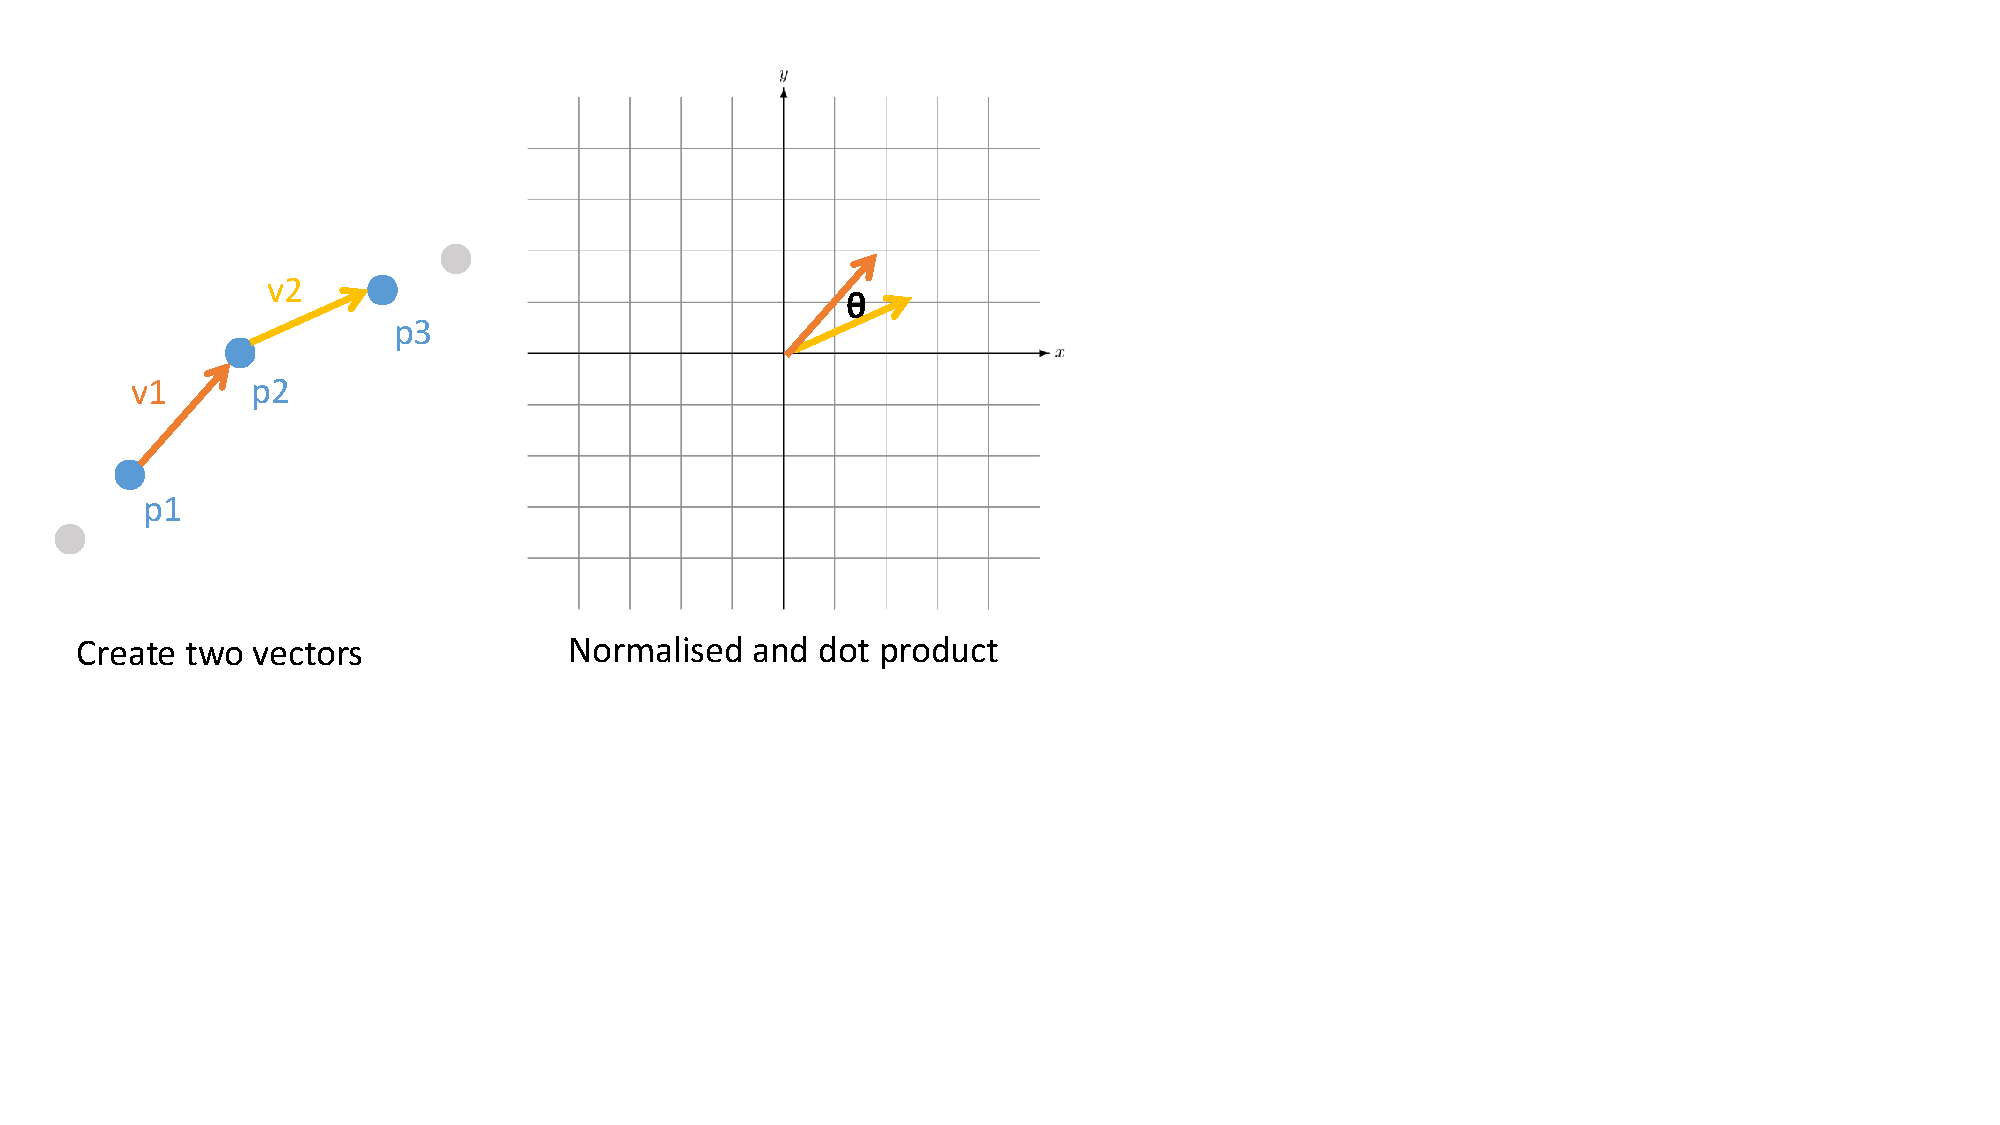
\includegraphics[width=\textwidth]{diagrams/vectorCorners.pdf}
		\caption[Splicing using vectors]{Points and vectors visualised}
		\label{fig:diagram-vectorCorners}
	\end{figure}
	
	\item [Find the mid point of a corner] The mid point of a corner is the highest point of the corner as shown in the figure. The mid point is found by going through each point. A perpendicular vector 'vP' to the first point is calculated, then a vector list vL is created containing a vector for each point as such v[x] = vector(p[x].x, p[x].y) where x is the position of the point in the array. Finally each vector in vL has the dot product with VP computed. The vector with the highest dot product result corresponds with the point which is the mid point of the corner.
	
	\begin{figure}[!htb]
		\centering
		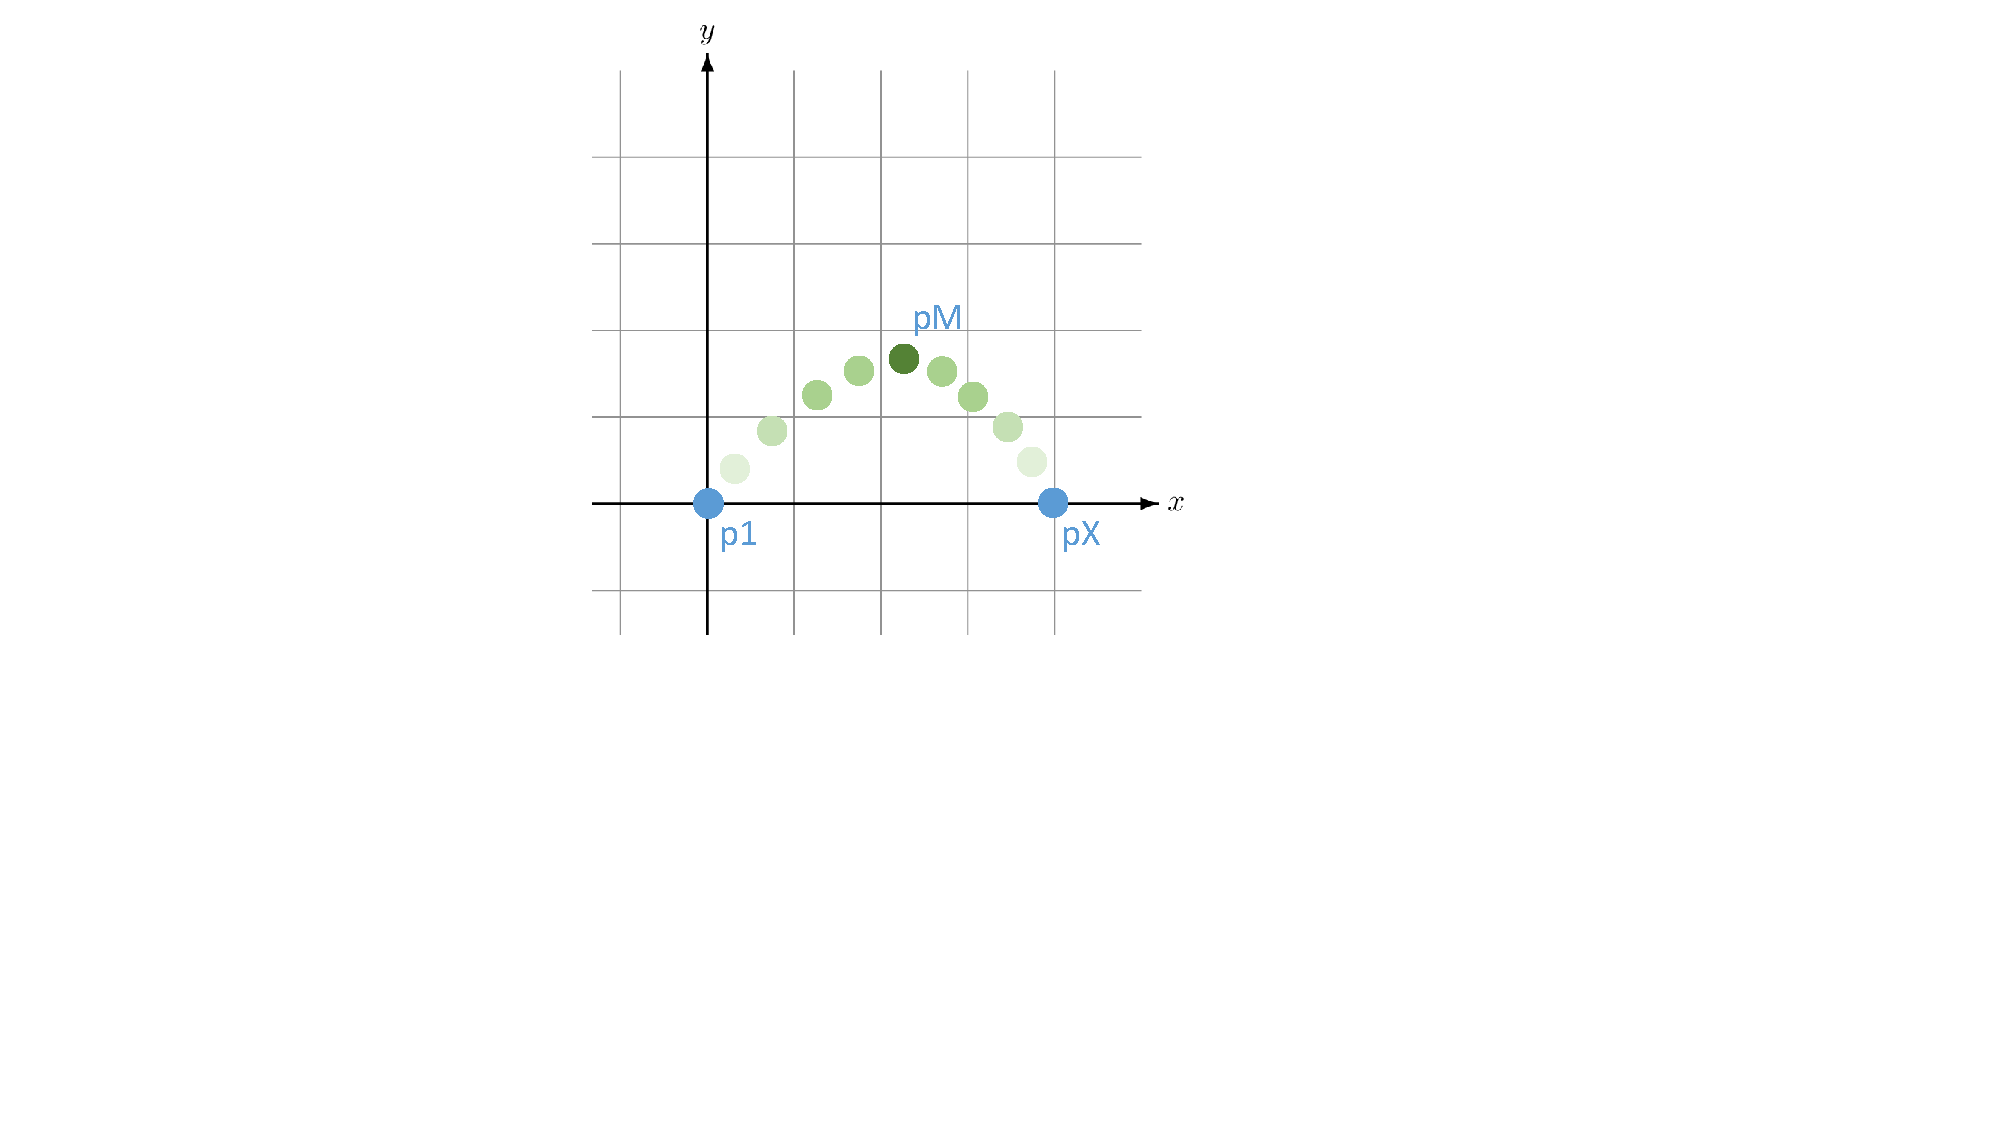
\includegraphics[height=5cm]{diagrams/cornerMidPoint.pdf}
		\caption[Corner mid point]{Finding the corner mid point}
		\textbf{p1} : First point \textbf{pM} : Corner mid point \textbf{pX} : Last point
		\label{fig:diagram-cornerMidPoint}
	\end{figure}
	
	\item [Visual representation of the race line] It was important to be able to visualise the results of the above processes in order to be able to determine the correctness of the processes. For this reasons an application with a graphic user interface was developed from which one can see the results.
	
	\begin{figure}[!htb]
		\centering
		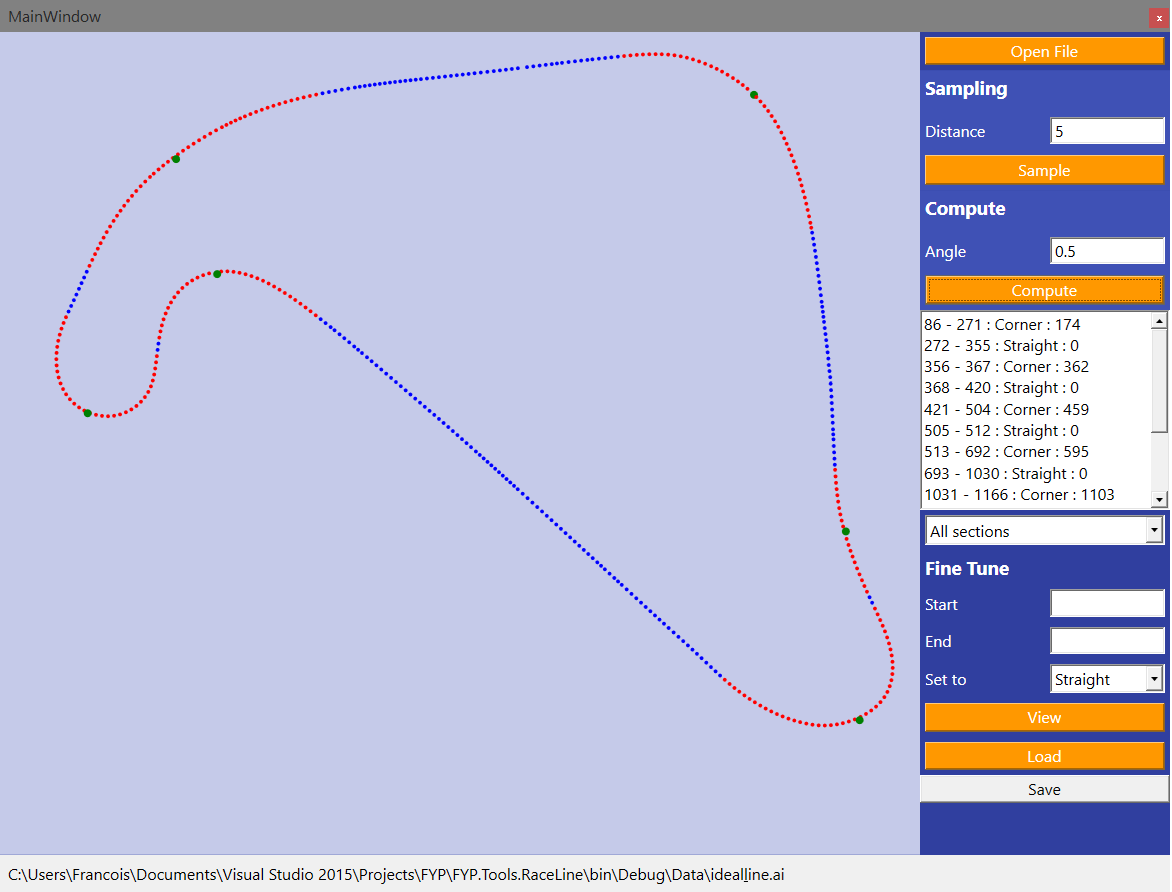
\includegraphics[height=5cm]{images/tracksplicertool}
		\caption{Track splicer tool}
		\textbf{Blue dots} : Part of a straight \textbf{Red dots} : Part of a corner \textbf{Green dots} : Corner mid point
		\label{fig:TrackSplicerTool}
	\end{figure}
	
\end{description}

\subsection{Persistence of Telemetry Data}
Log files containing telemetry data from each user session are inserted into a database management system for offline analysis. An extraction transfer loading (ETL) process (see Figure \ref{}) was purposely built, which takes as input a log file and inserts processed data as records into a database. This database is then used to run SQL queries related to the evaluation of the experiment.

\begin{figure}[!htb]
	\centering
	
\includegraphics[width=\textwidth]{diagrams/ssis.png}
	\caption{Microsoft Integration Services SQL import}
	\label{fig:ssis}
\end{figure}

\subsection{Spatial Queries}
\label{sec:imp-SpatialQuerying}
In order for \methodname to determine the closest point on the racing line from the car's current position a spatial querying mechanism is required. Since TeAR provides real-time feedback on how the user is following the racing line, spatial queries are continuously carried out. Therefore, rather than using a linear search, a quad-tree data structure \cite{} is used to store all the points on the racing line (see Figure \ref{}) and accelerate to $\mathcal{O}(\log{n})$ spatial queries. 

\begin{figure}[!htb]
	\centering
	
\includegraphics[height=5cm]{images/QuadTree}
	\caption{Visual representation for part of the quad tree for the Silverstone national circuit}
	\label{fig:QuadTree}
\end{figure}

\section{System Architecture}
\label{sec:imp-systemArchitecture}
The feedback system is made up of independent components which pass data to each other in order to produce the feedback instruction which is output to the user. Below is the break down of each component including an overview of their inner workings.

\begin{figure}[!htb]
	\centering
	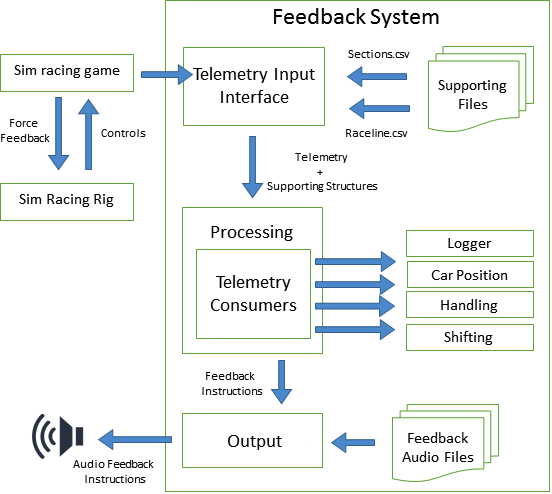
\includegraphics[height=10cm]{images/SystemArch}
	\caption{Overview of the system architecture components}
	\label{fig:SystemArch}
\end{figure}

\subsection{Telemetry Input Interface}
This components handles data inputs, two type of inputs are required, static and real time inputs. The static inputs are the ones which have been previously generated by the supporting tools. Real time input refers to the telemetry generated from the sim racing game. Assetto corsa provides a UDP server which a client can connect to, once the connection is established the game will send telemetry data.

\subsection{Processing}
Feedback processing is split into sub modules. Each module runs on a separate independent thread and gets a copy of the telemetry data passed in real time as it becomes available. Modules can be developed and plugged in without changing any other components. Having each module run on a dedicated thread ensures the system can scale horizontally making uses of all the available cores without hindering the feedback systems responsiveness. The processing component acts as a coordinator by passing data to sub modules, and listening to any feedback notification raised which are forwarded to the output interface.

\begin{figure}[!htb]
	\centering
	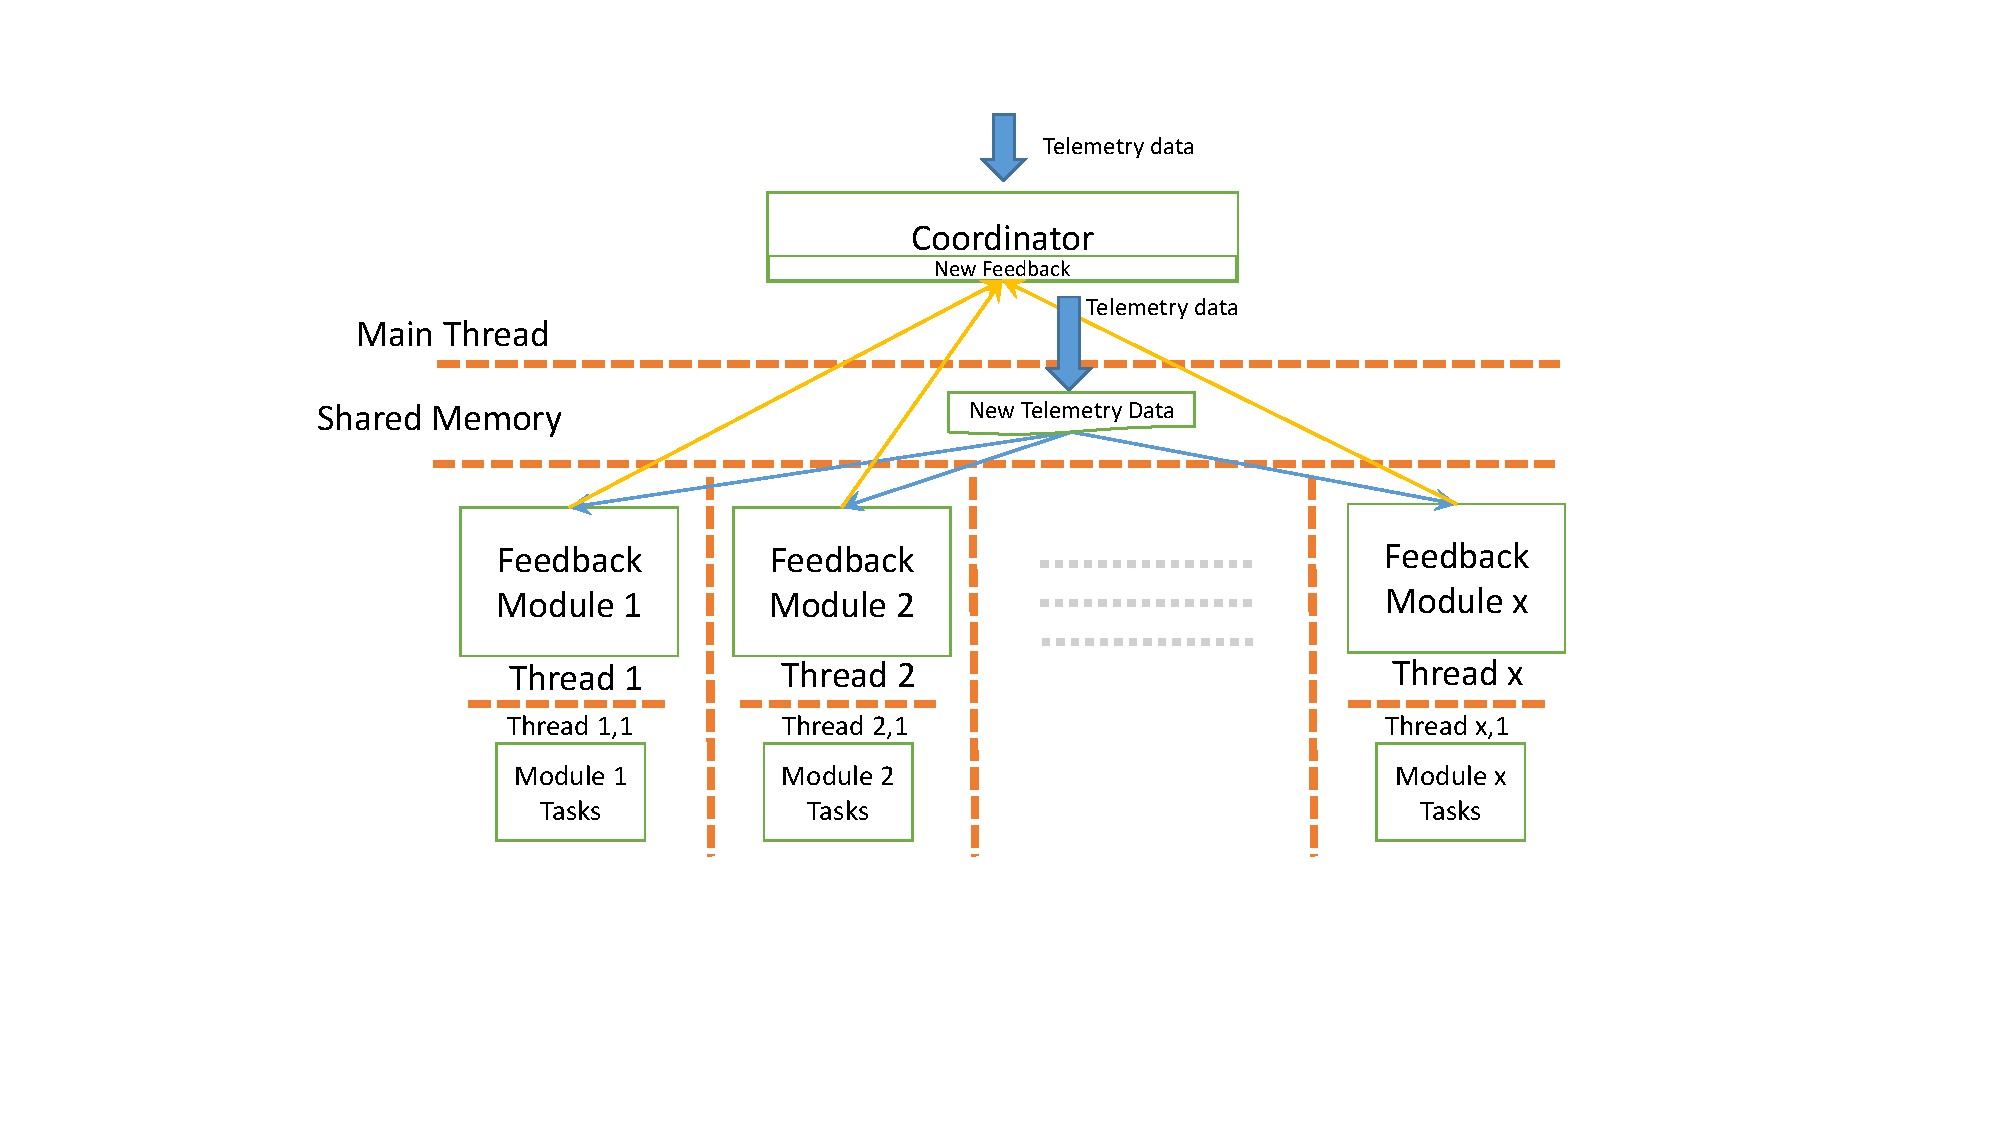
\includegraphics[width=\textwidth]{diagrams/multithreading.pdf}
	%[height=7cm]{diagrams/multithreading.pdf}
	\caption{Overview of the coordination threading}
	\label{fig:multithreading}
\end{figure}

Optimisation is also carried out within this component. This is achieved by filtering out by an expert system the feedback before being propagated to the output module. The knowledge base of the expert system is a hand crafted static one, based of rules and facts derived from the Background chapter. The inference engine works in a tiered skill based manner. At first only instructions from the basic tier are given. After the user manages to improve the basic tier skills, feedback instructions for the next tier are allowed pass to the output. In addition each module has a tolerance associated to each feedback notification it can provide. This allows the expert system to adjust how strict a module should be in raising a notification and be able to gradually make the system stricter as the user improves.

\subsection{Feedbacks being provided}
In this sub section an overview of all implemented feedback modules is given.

\textbf{Handling} component monitors for braking and acceleration behaviours. It is able to raise the following feedback notifications, 
\begin{itemize}
	\item Braking too hard
	\item Braking too light
	\item Braking in corner
	\item Losing traction to the drive wheels by applying too much power
\end{itemize}

\textbf{Car Position} component monitors for any issues which might cause the user to not adhere to the race line. As such this module can raise the following notifications 
\begin{itemize}
	\item Incorrect race line during corner
	\item Being too aggressive during a corner
	\item Not slow during a corner
	\item Track section report
\end{itemize}

\textbf{Shifting} component monitors how the user is changing gears, which allows it to raise the following notifications
\begin{itemize}
	\item Changing gear to soon
	\item Changing gear to late
	\item Taking too long to transition from one gear to another
\end{itemize}

\subsection{Output Interface}
Each possible feedback instruction which can be generated by the processing module has a static audio file associated to it. The audio files are generated from a free on line text to speech tool. The purpose of this component is to listen for feedback instruction generated by the processing component and play the corresponding audio file.

TO ADD How the logic of the feedback modules

\newpage
\chapter{Evaluation}
This chapter provides an insight into the data collected from the questionnaires and the feedback system logs while also explaining results derived from statistical tests. The chapter is structured as follows: \S~\ref{sec:eval-demographic} provides an over of the demographic background for the sampled participants. \S~\ref{sec:eval-distTests} covers test which check the data sets distribution moving on to compare the distribution across the feedback group and base group. \S~\ref{sec:eval-feedbackSysResults} goes through determining any difference between the two groups which might have been cuased by the introduction of the feedback system.  \S~\ref{sec:eval-usersFeedback} covers the participants impressions on the experiment and finally conclusive results from this study are presented in \S~\ref{sec:eval-Discussion} 

\subsection{Sim Racing Rig}
\label{sec:imp-simRacingRig}
The rig is made out of various independent components. The steering wheel is a Logitech G25 a pedal set, an H shifter and a bucket racing seat, all mounted on to a home made metal frame.

\begin{figure}[!htb]
	\centering
	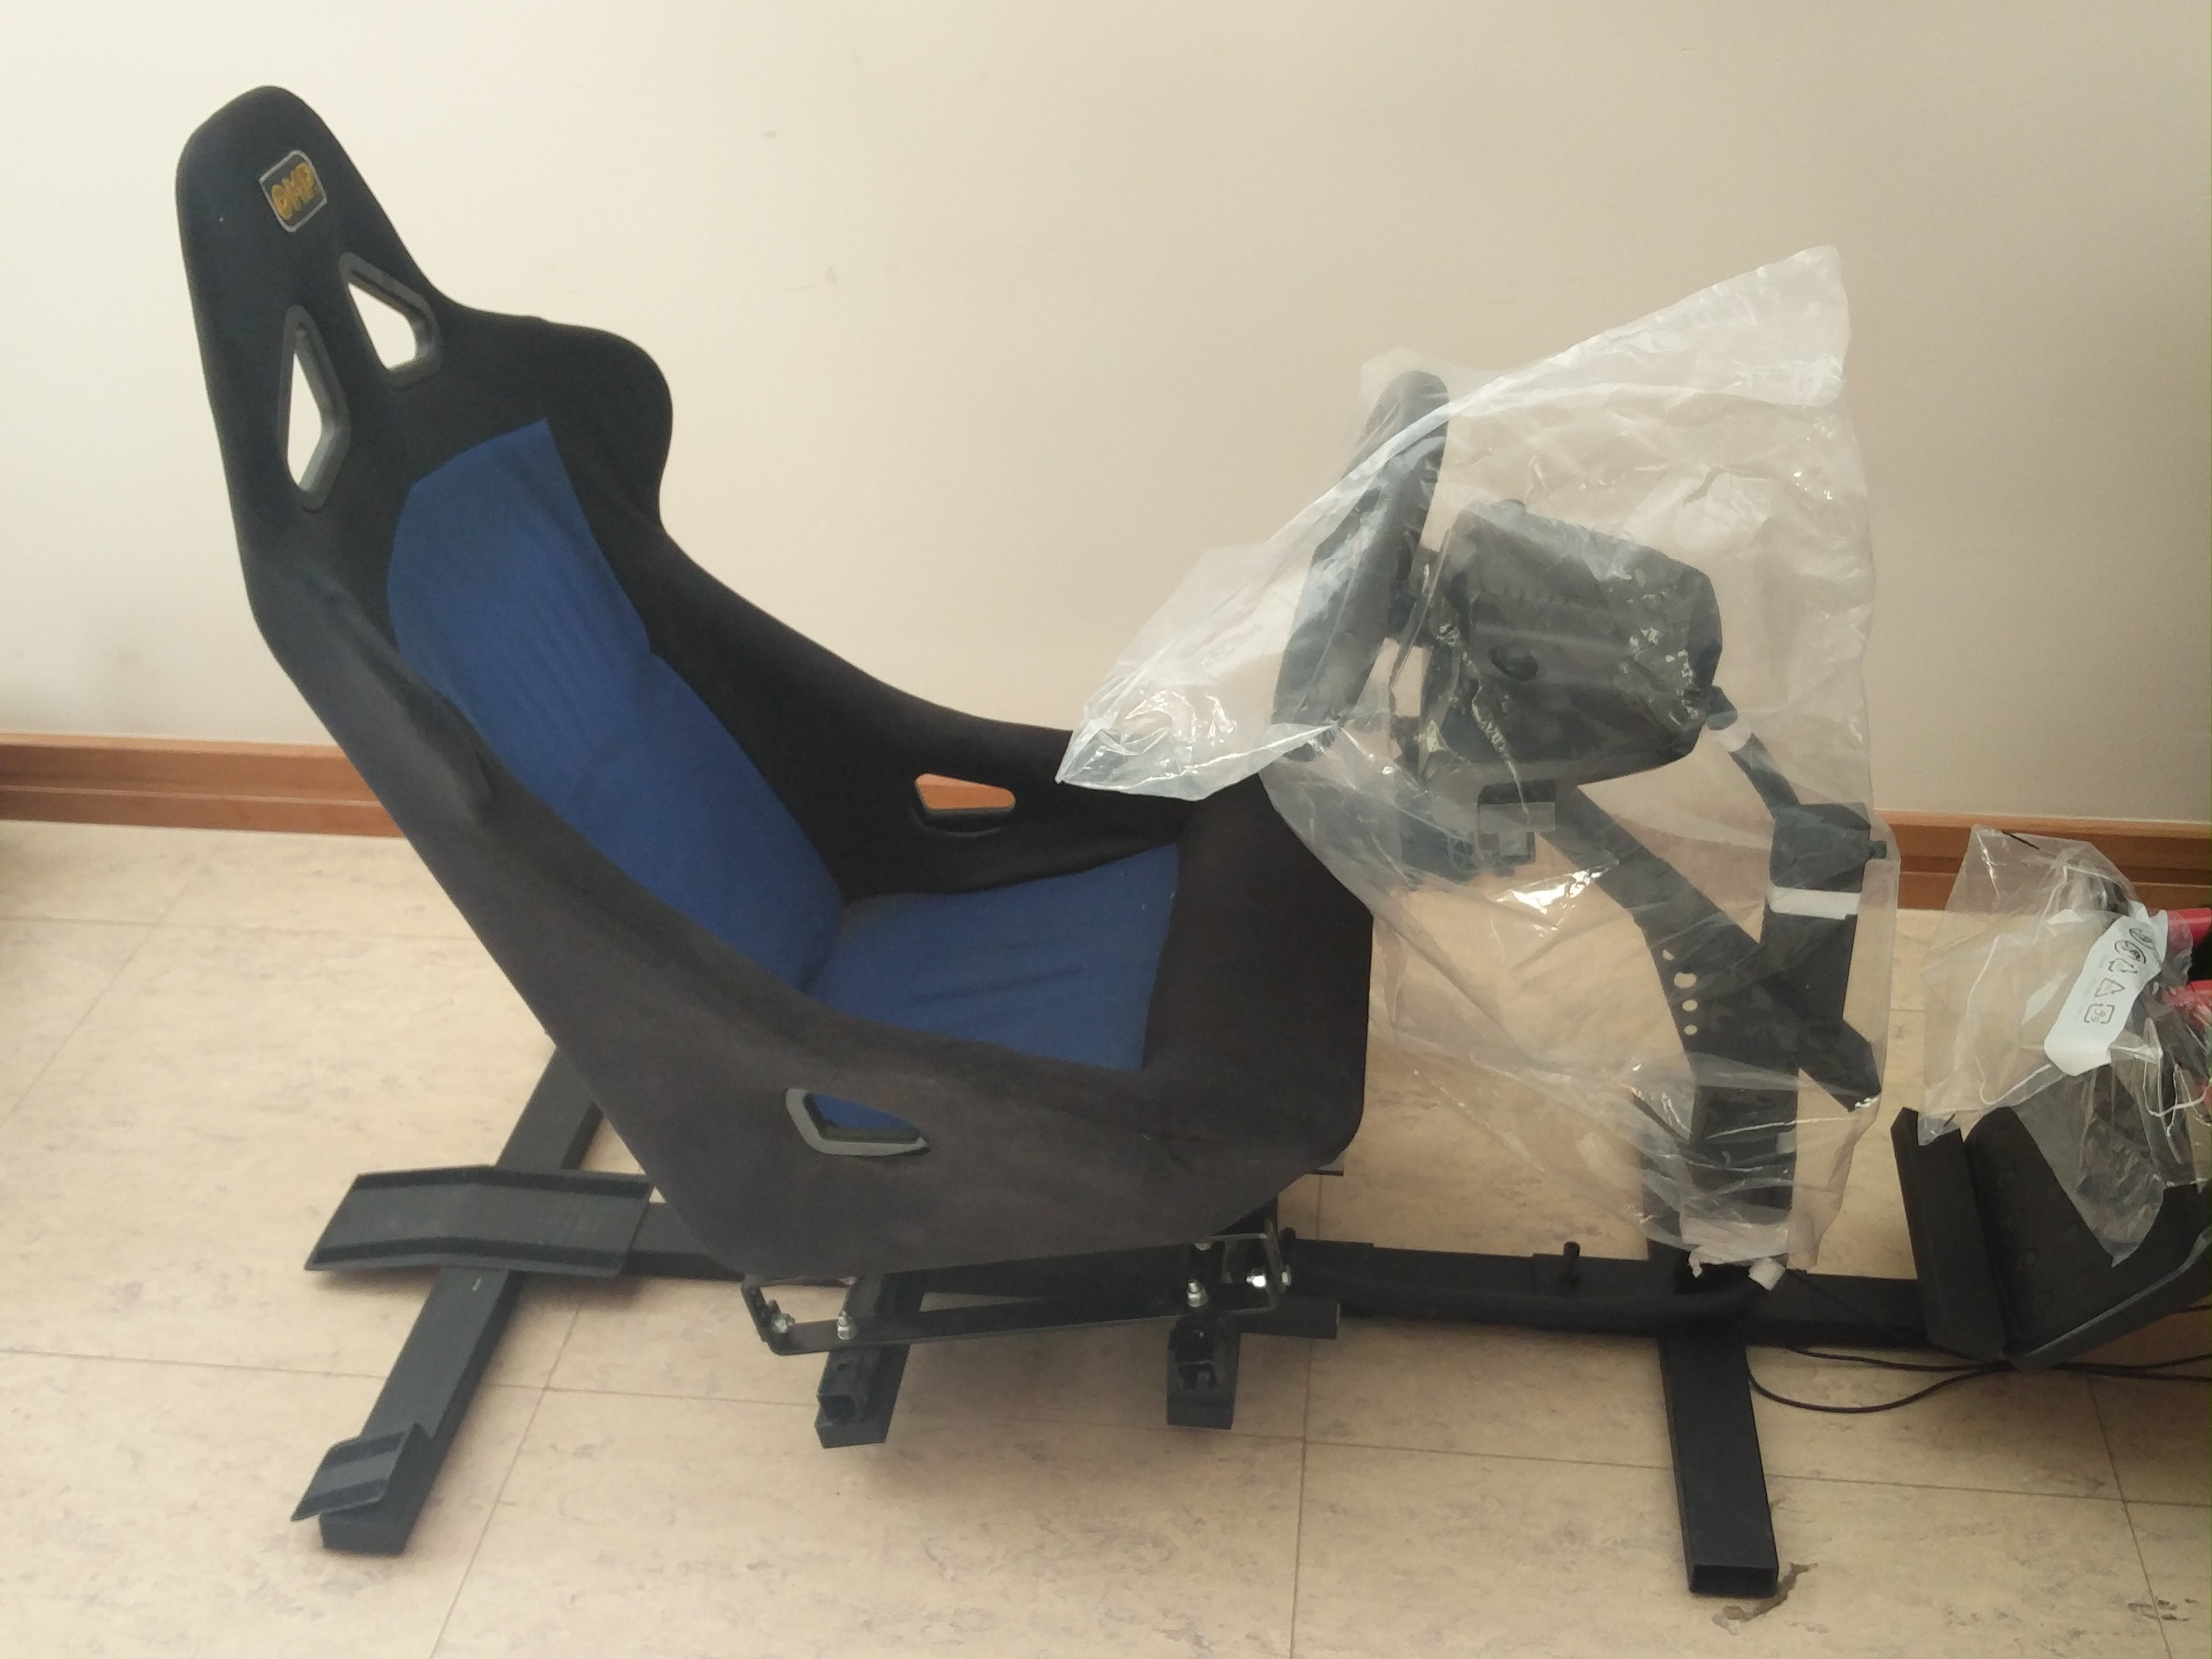
\includegraphics[height=5cm]{images/RacingRig}
	\caption{Side view of the racing rig}
	\label{fig:RacingRig}
\end{figure}

\begin{figure}[!htb]
	\centering
	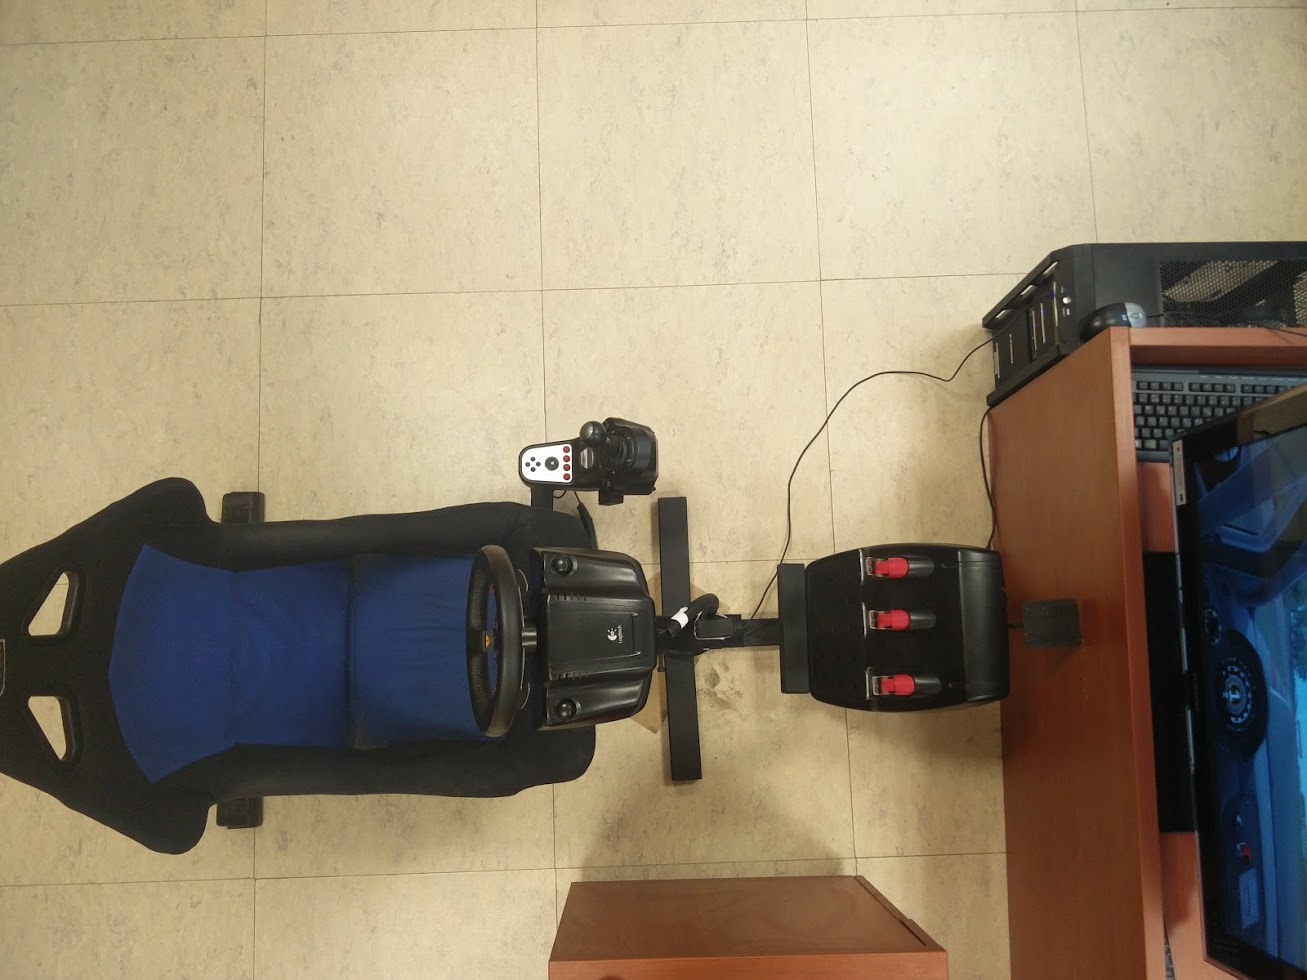
\includegraphics[height=5cm]{images/RacingRig2}
	\caption{Top view of the racing rig}
	\label{fig:RacingRigBirdsEye}
\end{figure}

\section{Demographic of The Sample}
\label{sec:eval-demographic}

The following demographic data was drawned out from the pre study survey. Participant's were mostly in their early twenties and mostly males. Out of 27 participants, 2 didn't have a driving license and 25 had a driving license with most of them have been driving for a year. Furthermore 22 participants identified them self as playing videos games, from which 18 participants stated they have played racing video games. The majority of participants who plays racing games identified them self as playing mostly arcade sim racing games, while only 3 play sim racing games. Out of the 27 participants, 7 participants have previously used a racing rig.

%I included the charts in the appendices as I didn't feel like they were adding much over here ending up just taking space.

\begin{figure}[!htb]
	\centering
	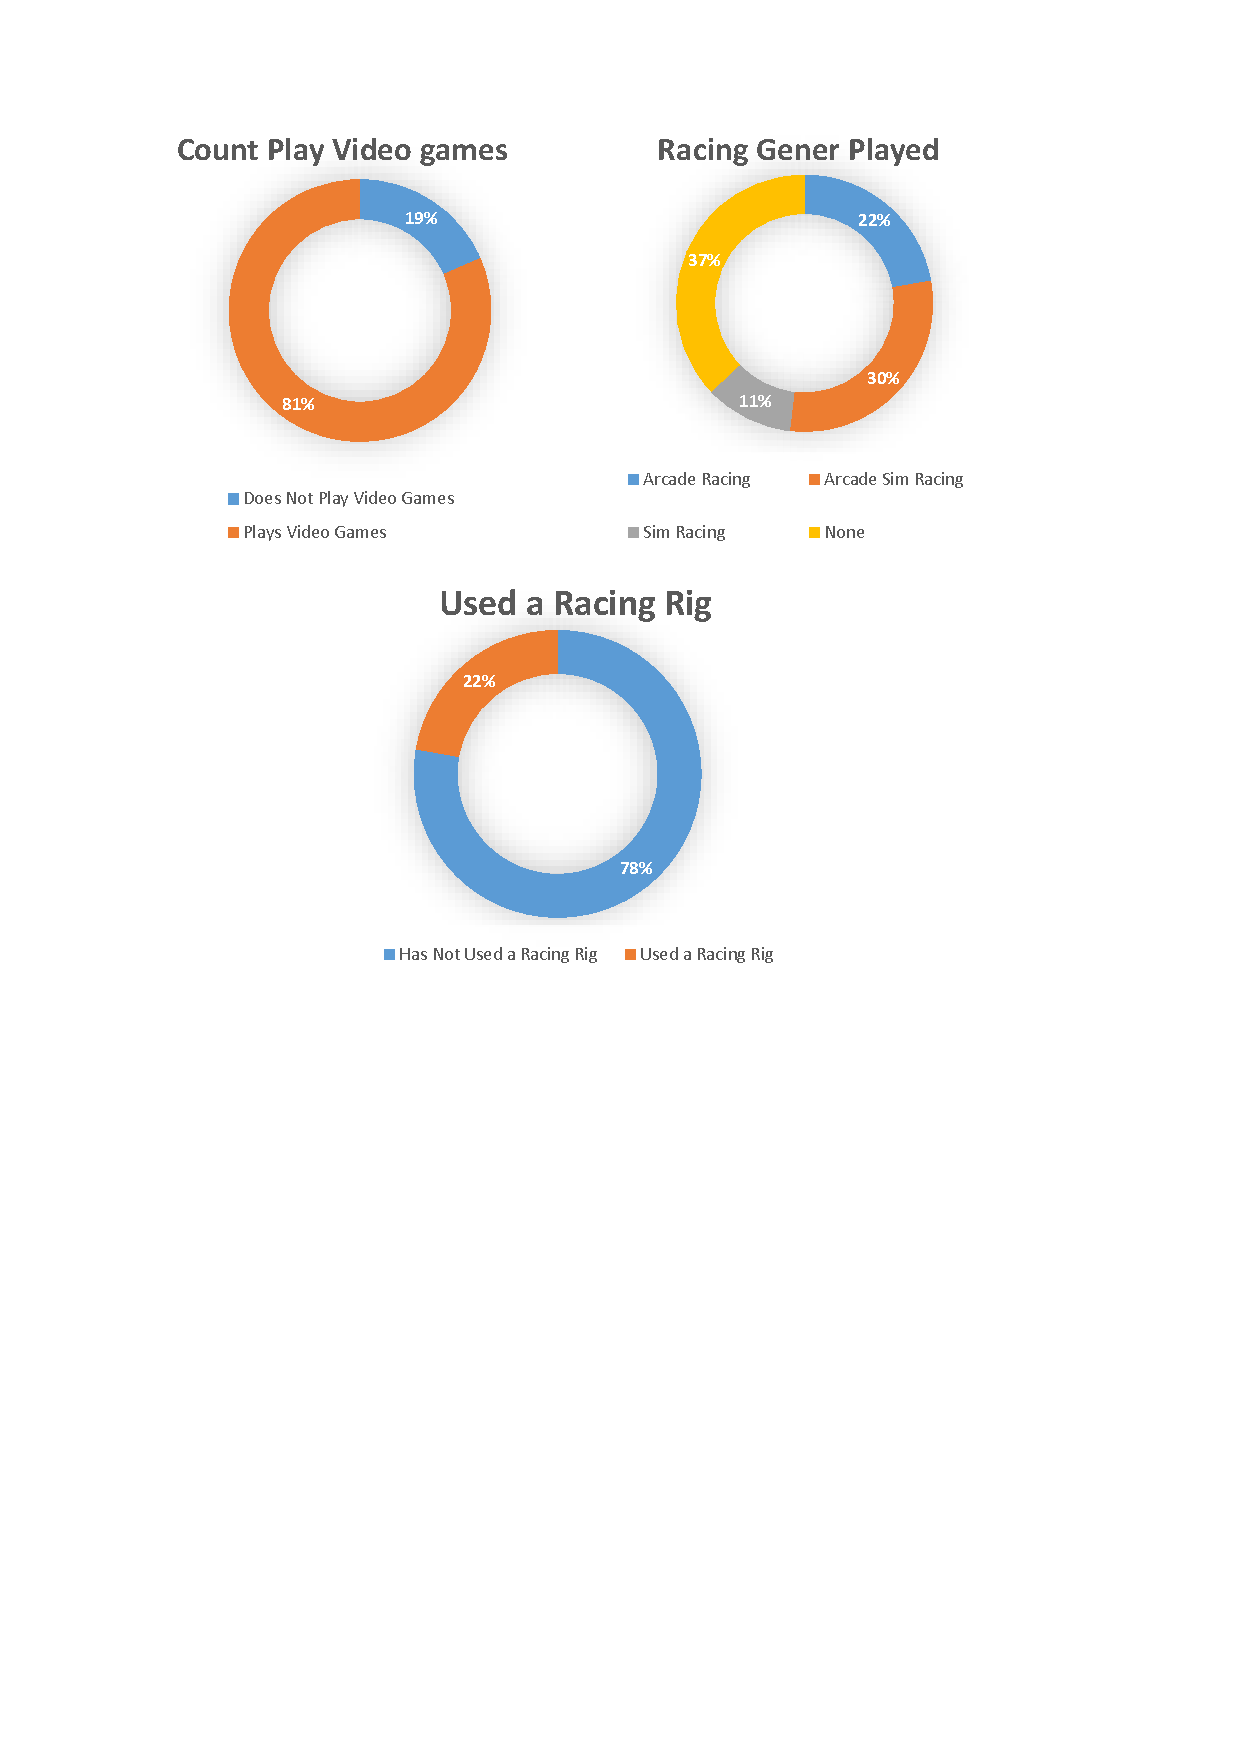
\includegraphics[height=10cm]{charts/gamesxp.pdf}
	\caption[Gaming xp]{Video games experience}
	\label{fig:chart-gamesxp}
\end{figure}

\section{Distribution Tests}
\label{sec:eval-distTests}

From the lap times box plot, one can notice a trend in which lap times improve the more time they use the rig, irrespective of the group assignment. It's worth pointing out the median of the feedback group is lower than the base group's median, except during the last session in which the medians are close to each other. Moreover the participants in the feedback group seem to be less consistent in their lap times as the box plot whiskers and quartiles are more spread out then the ones from the base group.

\begin{figure}[!htb]
	\centering
	\includegraphics[width=\textwidth]{charts/laptimes.png}
	\caption{Lap times vs session, clustered by group}
	\label{fig:chart-laptimes}
\end{figure}

Carrying out Shapiro-Wilk test for normality for the feedback group and base group during the first session on their respective lap times it was found that the data is not normally distributed as the p-value for both groups is below 0.05 resulting in rejecting the null hypothesis stating the samples come from a normal distribution

\begin{figure}[!htb]
	\centering
	
\includegraphics[width=\textwidth]{charts/shapiroWilkResults.pdf}
	\caption[Shapiro Wilk]{Shapiro Wilk test results}
	\label{fig:chart-shapiroWilk}
\end{figure}

The same data was checked for similar distribution across groups using the Independent Samples Kolmogorow-Smimov Test which resulted in accepting the null hypothesis stating the groups' lap times share the same distribution.

\begin{figure}[!htb]
	\centering
	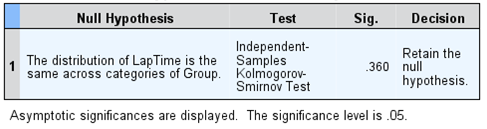
\includegraphics[width=\textwidth]{images/KolmogorowSmimov.png}
	\caption[Kolmogorow Smimov Test]{Kolmogorow Smimov test result}
	\label{fig:chart-KolmogorowSmimov}
\end{figure}

\section{Feedback System Results}
\label{sec:eval-feedbackSysResults}

Having established both groups' lap times share the same distribution during the first session the Mann-Whitney Test to determine any differences between the groups before the feedback system is introduced. The test results show a p value of 0.057 resulting in no statistical difference between the groups at the start of the sessions.

\begin{figure}[!htb]
	\centering
	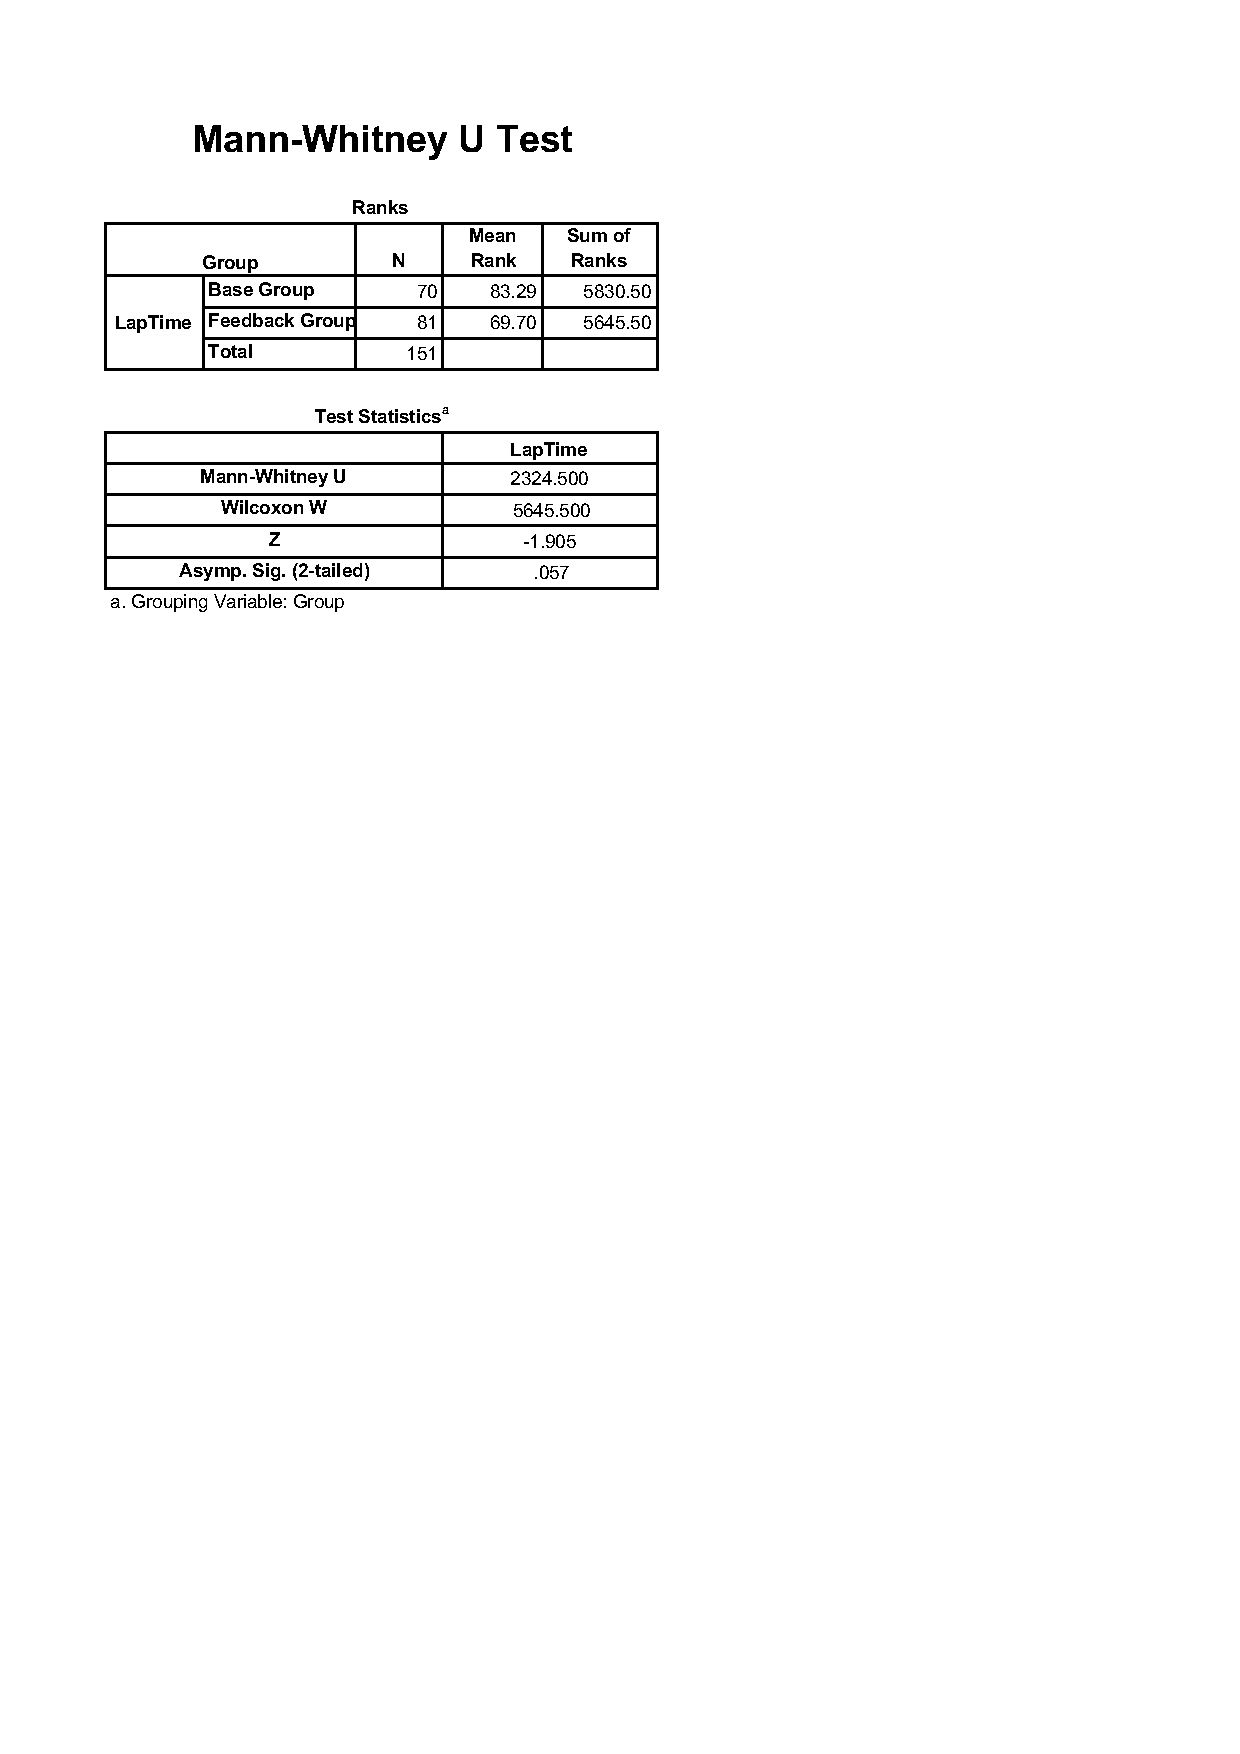
\includegraphics[width=\textwidth]{charts/Mann-Whitney.pdf}
	\caption[Mann-Whitney]{Mann-Whitney test result}
	\label{fig:chart-KolmogorowSmimov}
\end{figure}

Running the Mann-Whitney test on the remaining sessions, results show there is no significant difference between the two groups even after the feedback system was introduced to one group. The third session tells a different story as the p value is 0.029 which results is accepting the null hypothesis. The fourth and final sessions is the one which both groups had the feedback system turned off which resulted in the difference between the groups to yet again show no statistical significant difference.

\begin{figure}[!htb]
	\centering
	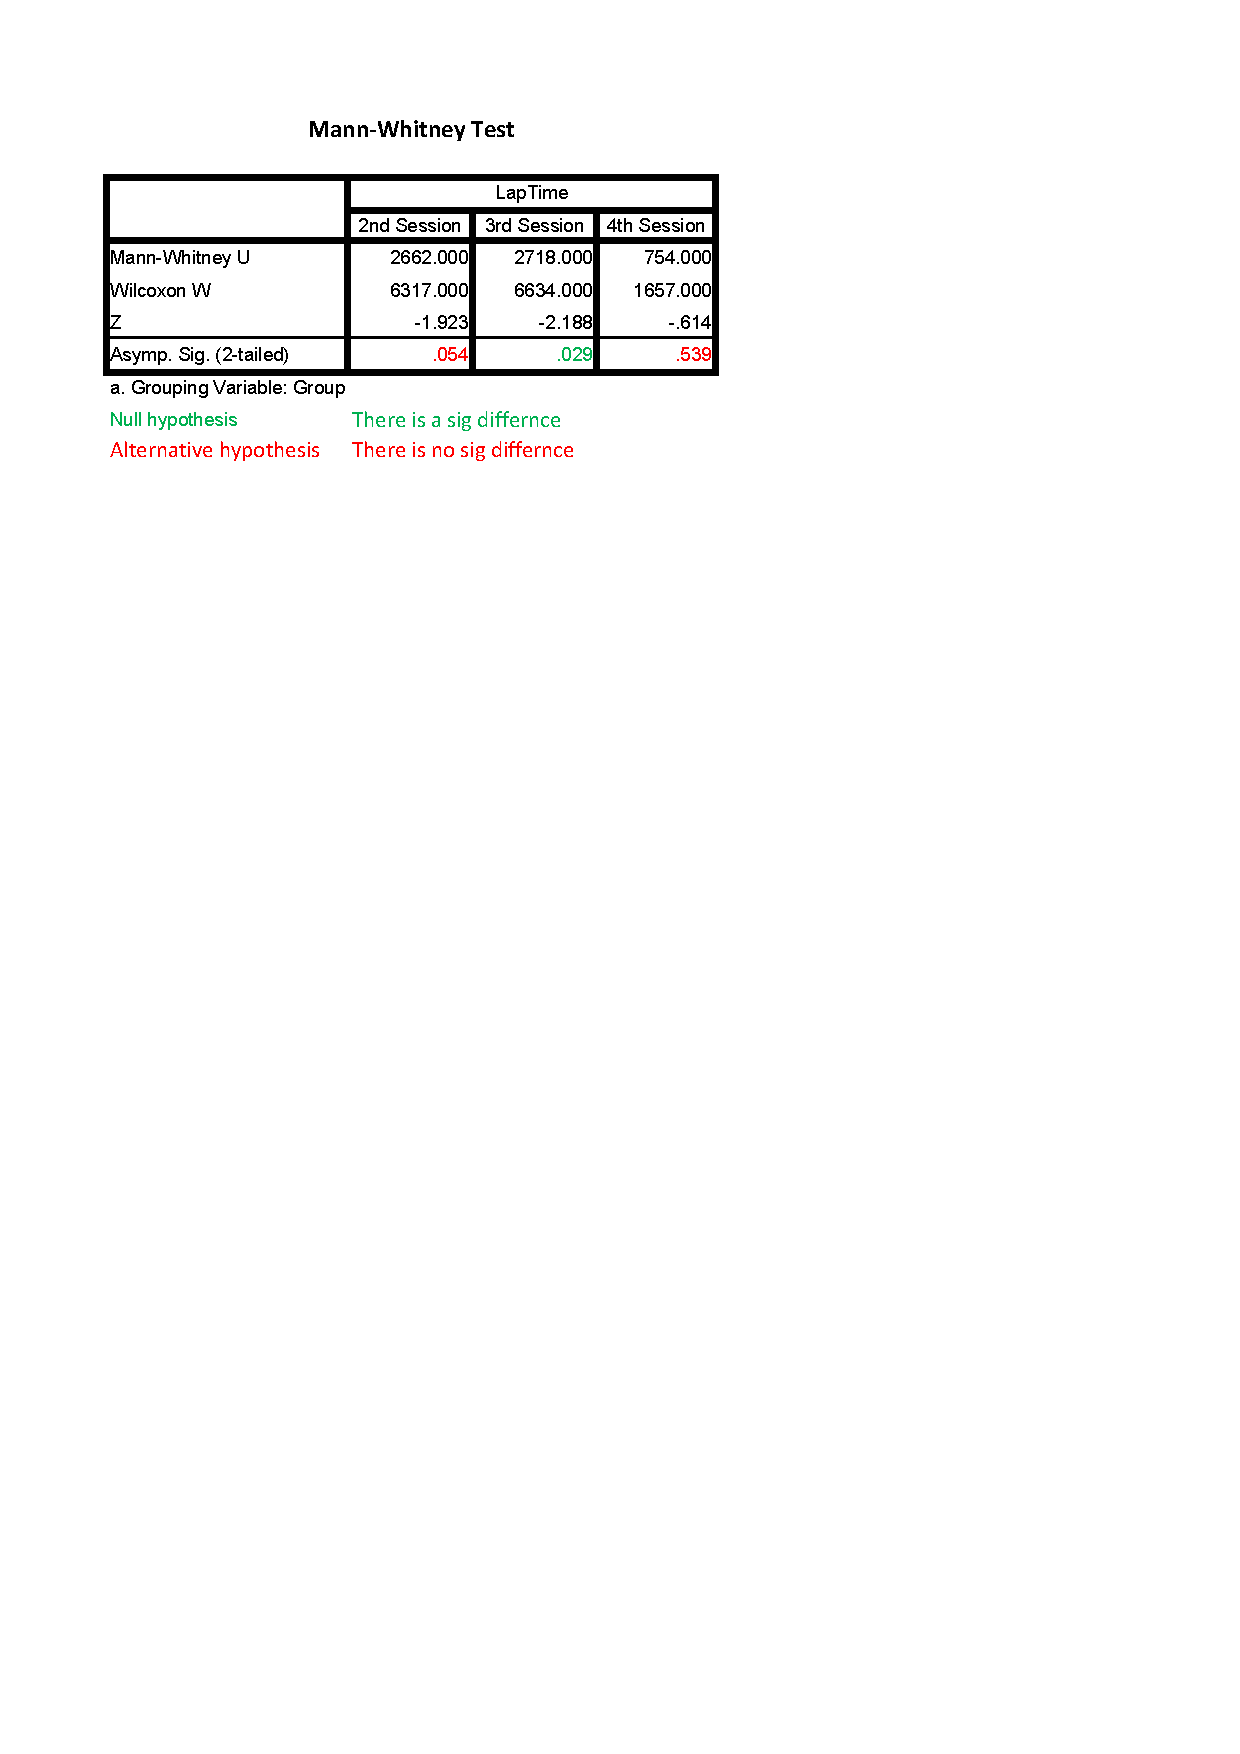
\includegraphics[width=\textwidth]{charts/Mann-Whitney-Sessions.pdf}
	\caption[Mann-Whitney Accross Sessions]{Mann-Whitney test result for the last the sessions}
	\label{fig:chart-Mann-Whitney-Sessions}
\end{figure}

\section{Users' Feedback}
\label{sec:eval-usersFeedback}

Users reported an overall good experience, the rig setup was found to be realistic and easy to use. An overwhelming majority of the participants reported having issues mastering the s-bend part of the track, however, they reported that the car and track choice was an adequate one. When the feedback group was asked about the feedback system, they reported to be intelligible, accurate, helpful and somewhat easy to apply the feedback given. Lastly, when asked about if the thought the feedback was intrusive, possible distracting them, out of 15, 5 reported it to be intrusive.

\begin{figure}[!htb]
	\centering
	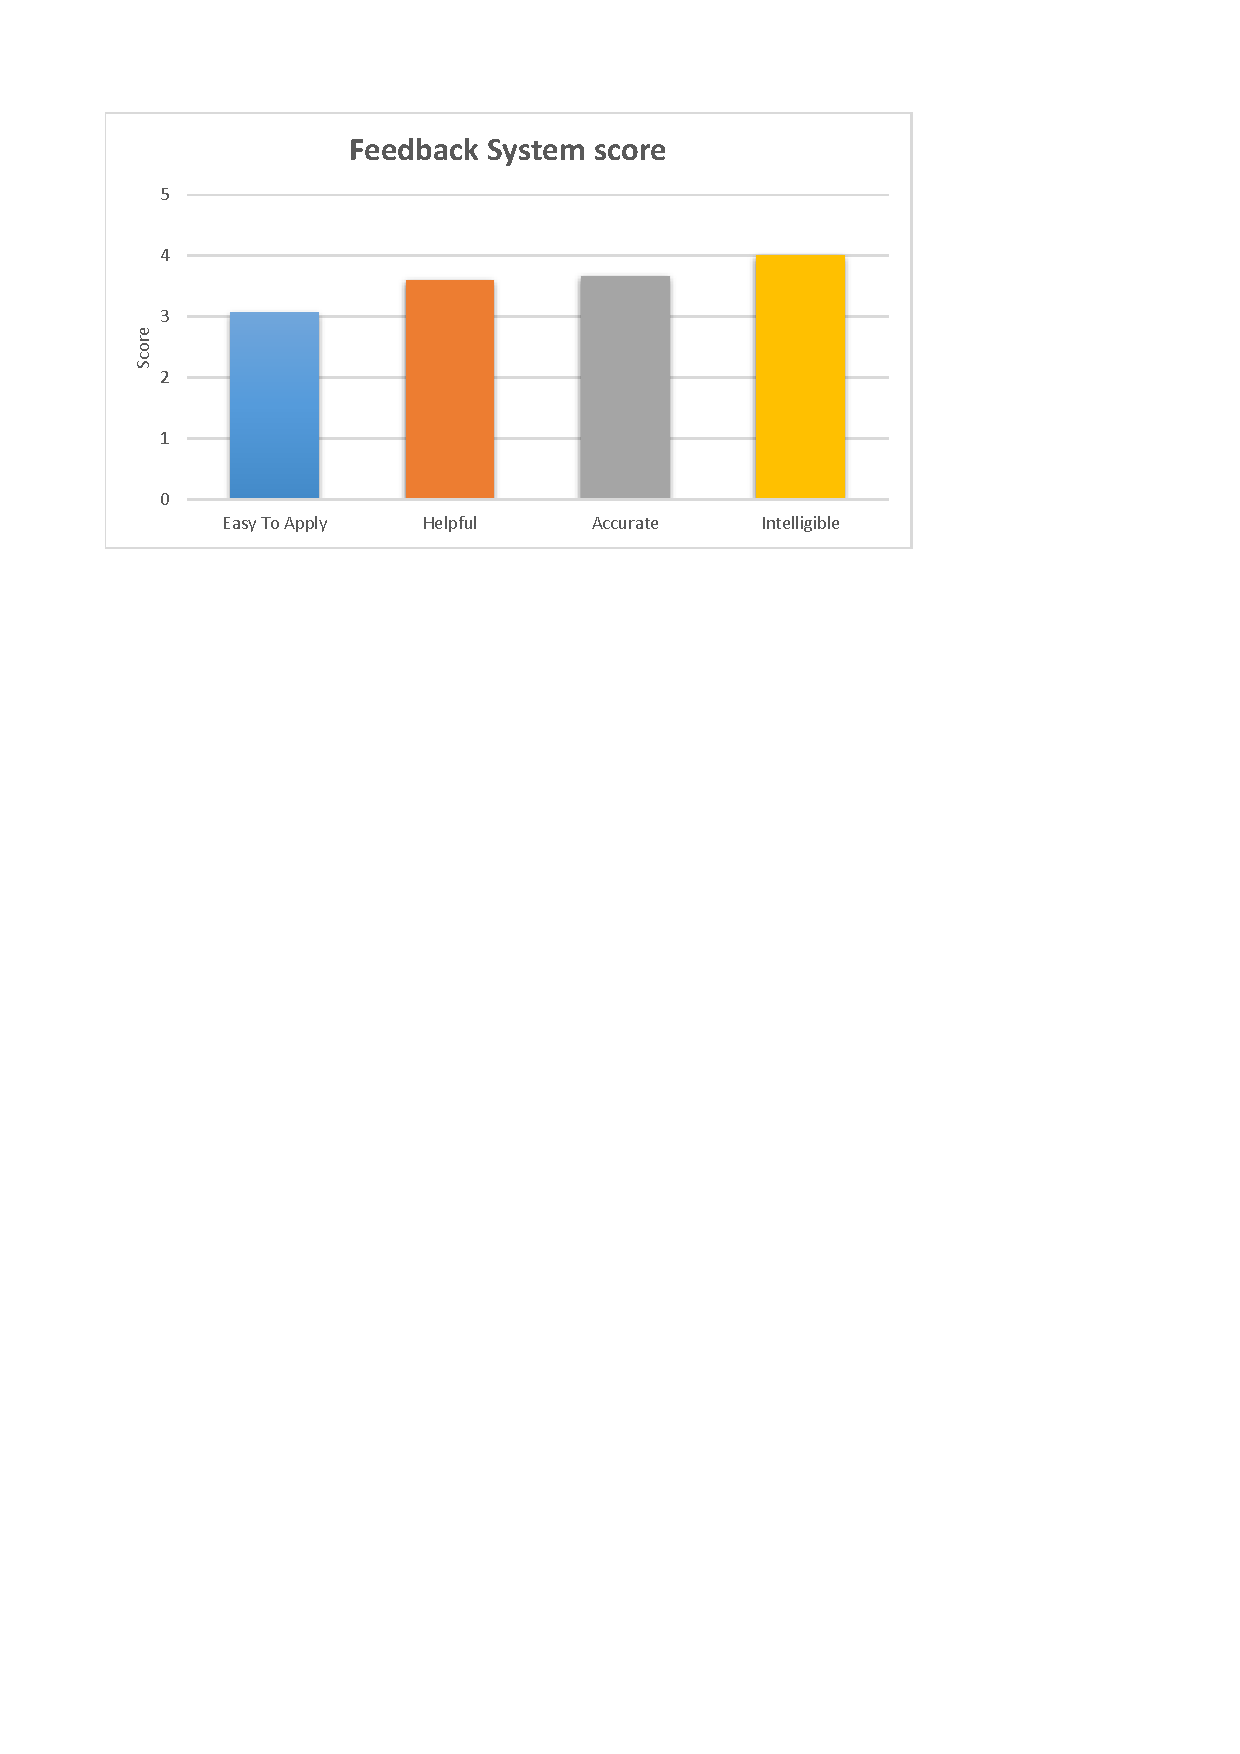
\includegraphics[width=\textwidth]{charts/feedbacksystemfeedback.pdf}
	\caption[feedback system feedback]{Users' Feedback}
	\label{fig:chart-feedbacksystemfeedback}
\end{figure}

\section{Discussion}
\label{sec:eval-Discussion}

From the post experiment questionnaire one can note that rig setup has been well received, with users enjoying the experiments while also given it a high score for it sense of realism. This suggests that by using off the shelf entry level hardware for the sim racing rig, it is possible to achieve a good level of realisem. the feedback system shows to have potential. the groups start of the same skill level. Both groups show a noticeable improvement from one session to the next session, excluding the last session in which it seems the shorter session might have but extra pressure on the participants' hindering their performance. Furthermore there was not statistical difference during the second session, but during the third session there was. The fact that the feedback group had a lower average lap time it suggest the group managed to get used to the feedback system after the second session and start to follow the feedback instructions during the third session. Lastly the sample is too sample to test for correlation between gaming experience and lap times, as only two players have played sim racing games while the other gamers don't play enough racing games. Same goes for correlation between having a driving licences and being able to the user the rig, as only two unlicensed participants took part, both of which are in the process of obtaining their driving license.

\newpage
\section{Future Work}

Having the feedback system control an AI car.
More data analysis
Observer the user for mistakes such as not keeping both hands on the wheel resting the hand on the shifter and not looking into a corner.

Teach users in the sim, have them drive in real life.

Whether by the end of the project all the original aims and objectives have been completed or not,
there is always scope for future work. Also the ideas will have grown during the course of the project
beyond what the student could hope to do in the time available. The Future Work section is for
expressing these unrealised ideas. It is a way of recording 'I have thought about this'. A good Future
Work section should provide a starting point for someone else to continue the work which has been
done. 

At present only negative feedback is given, a good idea would be to look into the benefits of letting the user know when a particular task has been completed correctly.

\newpage
\chapter{Conclusion}
The Conclusions section should be a summary of the project and a restatement of its main results,
i.e. what has been learnt and what it has achieved. An effective set of conclusions should not
introduce new material. Instead it should draw out, summarise, combine and reiterate the main
points that have been made in the body of the dissertation and present opinions based on them. 

\section{Future Work}

Although the results presented here have demonstrated promising results and the system could be further developed in a number of ways:

\subsection{Suggest positive feedback}
At present the system only output feedback whenever a user does something wrong, an improvement to the system could explore the possibility of letting a user know whenever a previous mistake has been corrected,

\subsection{Visual and auditory hybrid feedback}
One can also look into implementing a hybrid feedback system, in which auditory feedback is aided by visual elements on screen. An example of such feature could be showing a user the slip ratio while braking. This could aid the user to better fine tune the braking as users would have a way to actually see how far off they are from the optimal braking slip ratio.

\subsection{\methodname control an AI car}
At present \methodname is tailored to aid users, however one could modify the output to control an AI car. This would work as a combination of neural net and fuzzy logic. In which the neural net is thought how to drive via the feedback system and the fuzzy logic is used to control the car. In this case the output would need to map to actual car controls inputs such as steering and pedals.

\subsection{Observer participant’s behavior while driving}
During the experiments it was noted that some lacked based skills such as keeping both hand on the wheel, not crossing hands while turning the wheel and resting the hand of the shifter. These events were outside of the scope of this system, and could not be monitored using telemetry data. However, one could use motion tracking camera to capture and report on such behaviors. 

\subsection{Teach users in the sim, have them test in real life}
The ultimate experiment for such a feedback system would be to have a set of participants who are trained in a virtual environment and then have them proof their learned skills in a real life environment. This would further validate the case for a racing serious game being used to teach users how to race.

There is clearly much work to be done in the area of, racing simulators and serious games. Perhaps the most direct extension of this work is by the means of using
a exploring any possibilities to further improve auditory feedback which is being provided at present 

\newpage
\section{Glossary}

\newpage
\section{Appendices}
Transcript of the audio files

\newpage
\bibliography{citeations}{}
\bibliographystyle{plain}

\end{document}